

  This chapter provides explanations of the following technologies;
  1) Overlay network
  2) Multicore packet processing
  3) IPVS load balancer
  4) XDP technology.
  These are the underlying technologies used in this study, and knowledge of these is necessary to understand the contents of this thesis.





Overlay networks are used to deploy Kubernetes clusters in most cases in order to separate the node network and container network.
The author has also found that the choice of the operation mode \added[id=4th]{of the overlay bnetwork} greatly affects the throughput of the load balancers, as will be explained in Chapter~\ref{chapter:Performance Evaluation}.
Therefore, flannel, which is one of the overlay networks and is used in this study, is explained in detail.

Secondly, the author explains how to utilize multi-core CPUs for packet processing in Linux.
The Linux kernel comes with built-in features for multi-core packet processing.
However, the default setting of Linux distribution might not \replaced[id=4th]{be necessarily}{necessarily be} optimized for the best performance, which sometimes hinders the understanding of experimental results.
That was the case when the author first carried out the experiment, and therefore the author explains about it.

Thirdly, the author explains Linux kernel's IPVS load balancer, because IPVS is used to implement \replaced[id=4th]{the proposed}{a} load balancer in \replaced[id=4th]{this study}{a container}.
The IPVS has three \replaced[id=4th]{operation}{operating} modes\replaced[id=4th]{, and two of them used in this study}{ and they} are also explained.

Lastly, the author briefly explains about novel XDP technology.
The author plans to replace IPVS based load balancer with the one based on XDP technology in future work.
The author has already started the implementation of such load balancer and presents a preliminary result in Chapter~\ref{chapter:Further Improvement}.
The explanation of XDP technology is necessary to understand why it is supposed to be faster than IPVS.


\section{Overlay network}


  An overlay network is used to deploy a Kubernetes cluster in most cases in order to separate the node network and container network.
  %  It is also possible to let nodes and containers use the same network
  In the case of Kubernetes, every {\em pod}\footnote{A {\em pod} is a group of containers that share the same network namespace and cgroup, and is the basic execution unit in a Kubernetes cluster.} is assigned with its own IP address.
  If the administrator of Kubernetes cluster plans to host up to 10 {\em pod}s on a single node, roughly 10 times larger IP address space is required for container network than for node network.
  And if \replaced[id=4th]{one}{he or she} plans to host up to 100 {\em pod}s on a single node, 100 times larger IP address space is needed. 
  Therefore in practice, it is often convenient to separate administrations of node network and container network using overlay network.


\subsection{Container network}

There are several types of container network including, veth \cite{bhattiprolu2008virtual}, MACVLAN \cite{rathore2010performance}, IPVLAN \cite{ipvlan}, host network.
There are good reviews of these network in  \cite{Marmol2015,claassen2016linux,struye2017assessing}.
The author uses the container network that uses \added[id=4th]{bridge and} veth because of the popularity and easiness of the setups.
Here the setup used in the experiments is explained.

Figure~\ref{fig:bridge+veth} shows a schematic diagram of the container network used in this study.
The veth kernel module creates a pair of network interfaces that act like a pipe.
One of the peer interfaces is kept in the host network namespace and the other is added to the container namespace.
The interface in the host network namespace is connected to a network bridge\added[id=4th]{, docker0}.
In the case of Docker, most of the veth setup is done by the Docker daemon.

The communication between two containers on the same physical node is through the docker0.
The communication with the outside of the node \added[id=4th]{further} follows the routing rules in the kernel,
and optionally \added[id=4th]{translated using} iptables Masquerade\added[id=4th]{ or Source Network Address Translation (SNAT) \cite{MartinA.Brown2017}}.  

\begin{figure}[h]
  \centering
  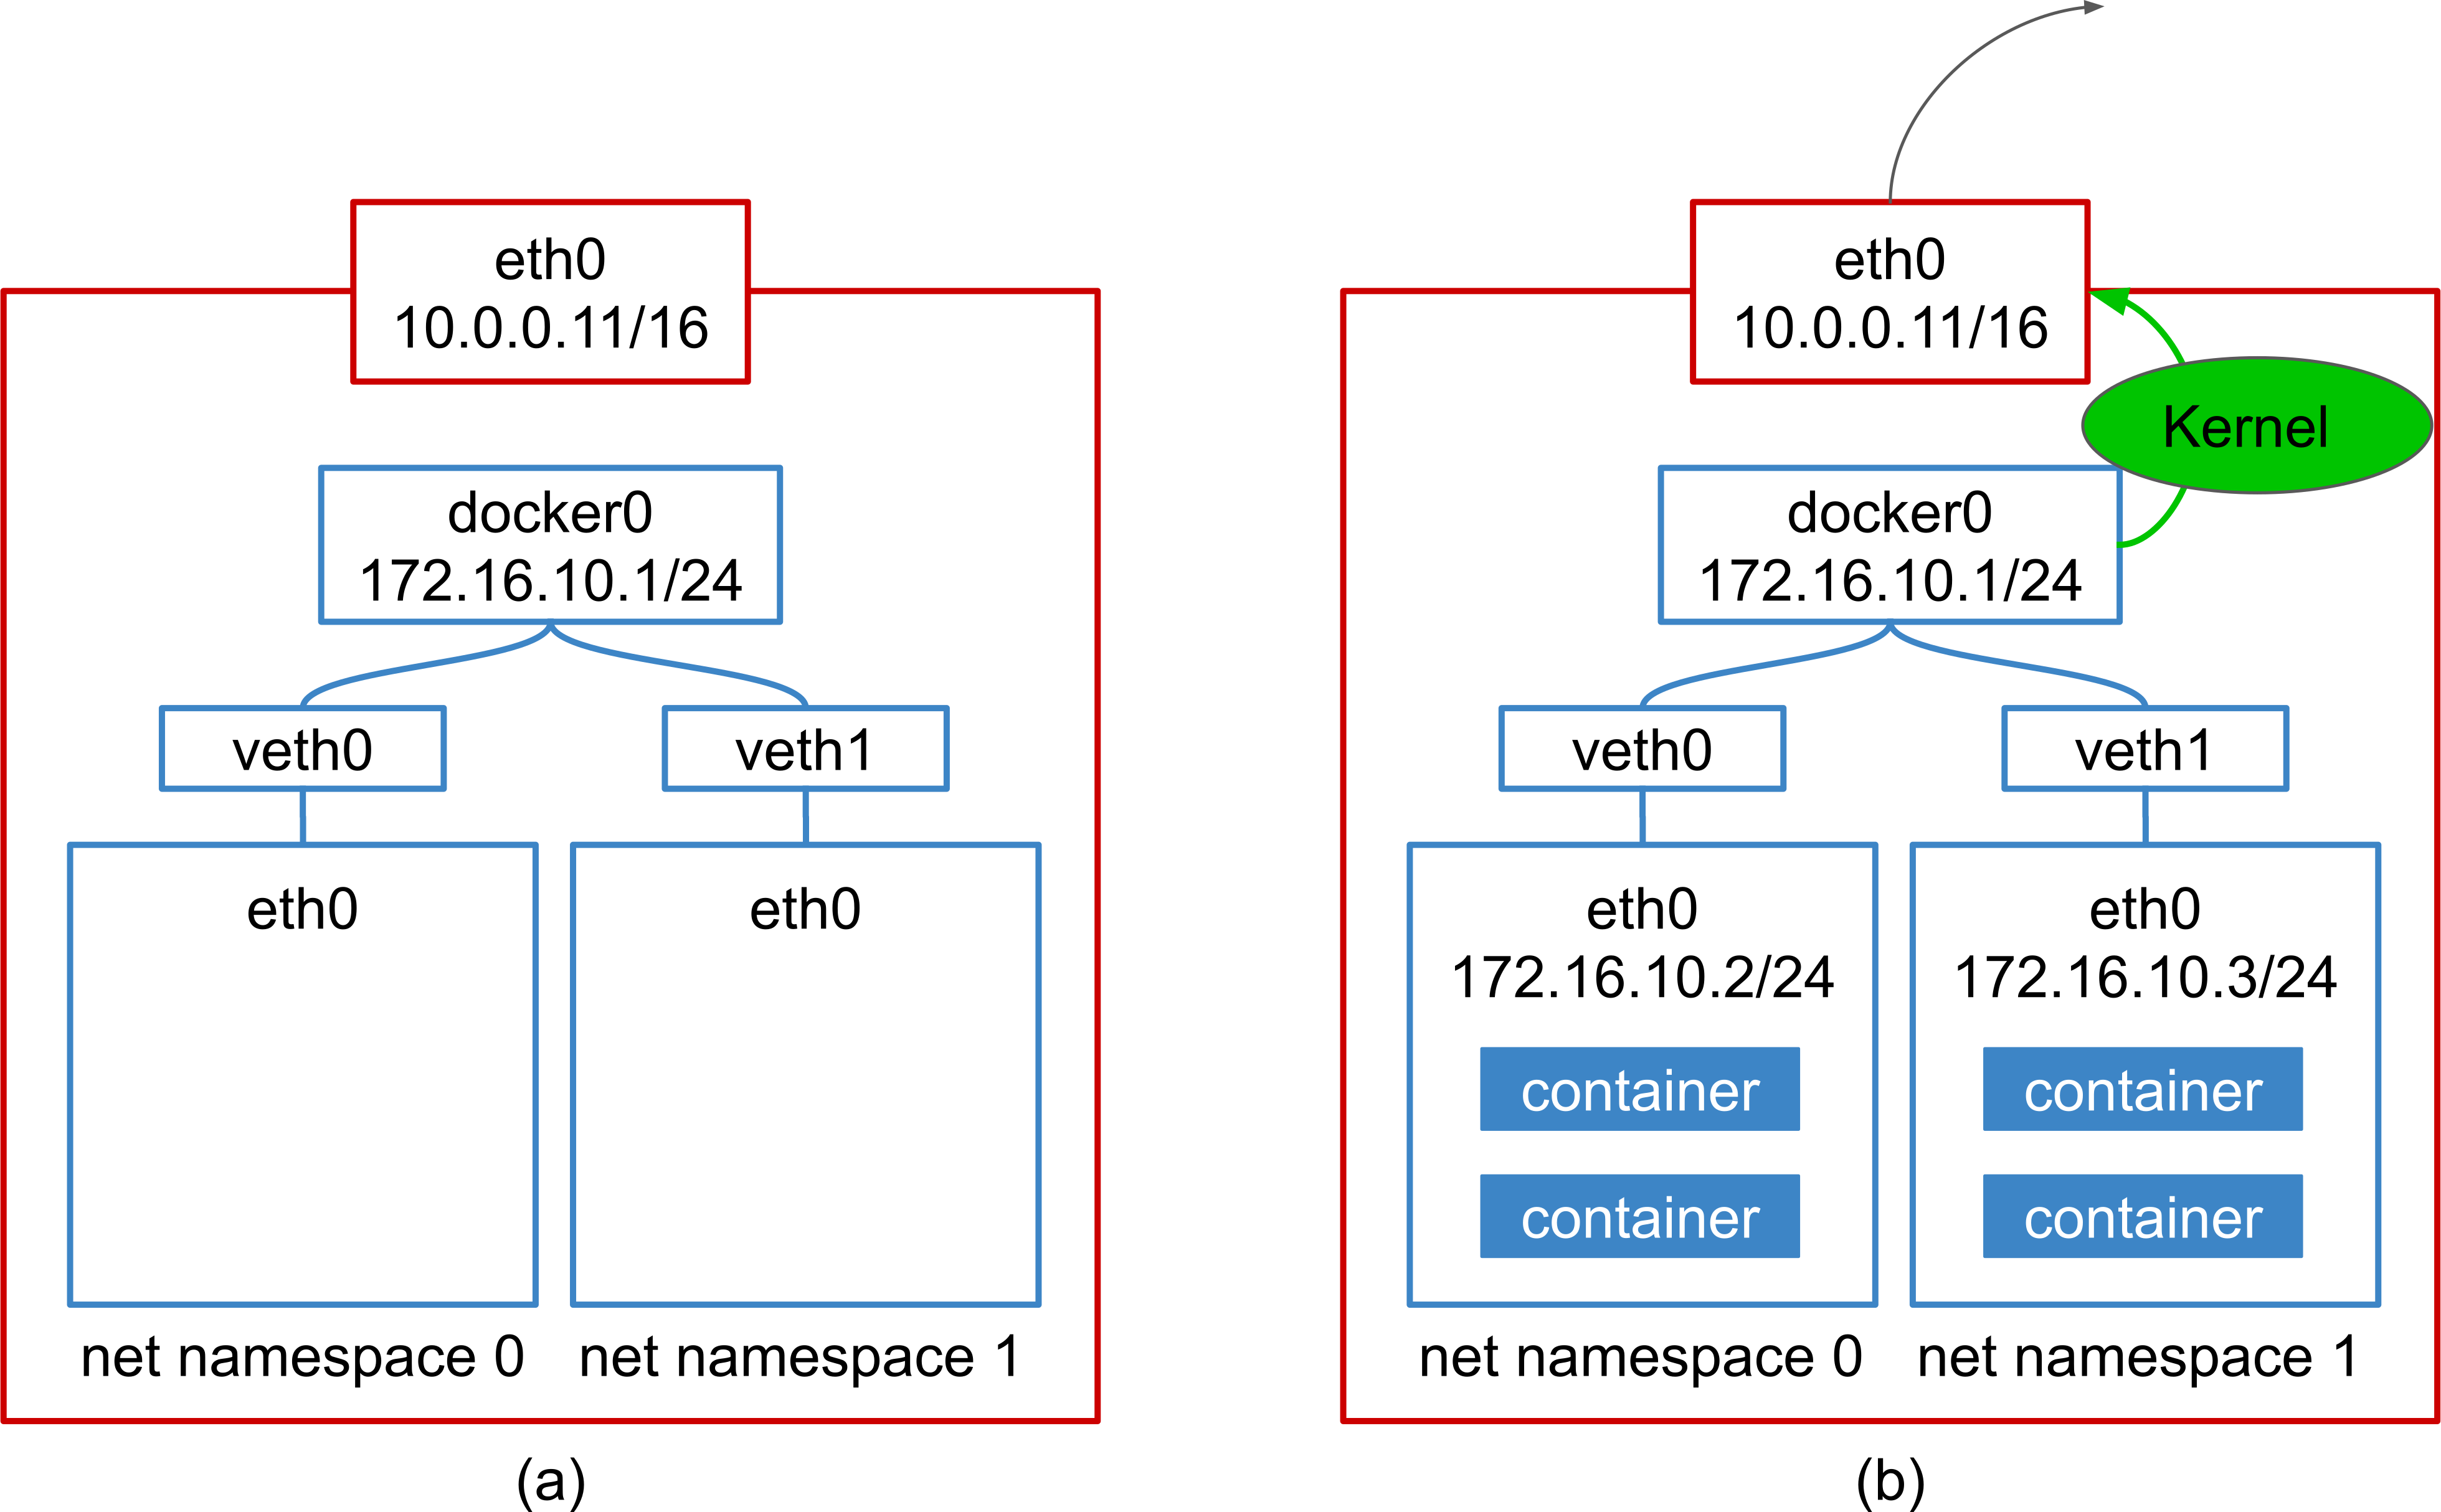
\includegraphics[width=0.95\columnwidth]{Figs/bridge+veth}

  \par\bigskip
  \centering
  \begin{minipage}{0.9\columnwidth}
    \caption[Docker networks setup]{
      Docker networks setup.
      \added[id=4th]{
      (a) Two pairs of network interefaces (veth0,eth0) and (veth1,eth0) are created.
      Each of the pairs acts like a pipe.
      The veth0 and veth1 are placed in the host (node) network namespace, and connected to the docker0 bridge.
      The eth0s are placed in respective container namespaces.
      (b) Communication between network namespace 1 and 2 is through the docker0.
      Communication with the outside of the node follows the routing table inside the kernel.
      }
    }
    \label{fig:bridge+veth}
  \end{minipage}
\end{figure}
 
When a container needs to communicate with other containers on different nodes, the kernel needs to know on which node the peer container exists.
The kernel normally does not know this, but if there is the help of overlay network \cite{zismer2016performance}, the kernel eventually finds out the next hop towards peer container.

\FloatBarrier

\subsection{Overlay Network}

%\subsubsection{Flannel}

\added[id=4th]{
There are several choices for the overlay networks with popular ones being flannel \cite{CoreOSFlannel}, calico \cite{ProjectCalico}, weave \cite{WeaveNet}, etc.
The author used flannel throughout this study because of its popularity and easiness.
}
\deleted[id=4th]{
The author used flannel to build the Kubernetes cluster used in the experiment.
}
Flannel has three types of backend, {\it i.e.}, operating modes, host-gw, vxlan, and udp \cite{CoreOSFlannelBackend}.
\added[id=4th]{
These are explained here.
}

\subsubsection{host-gw mode}

In the host-gw mode, the flanneld installed on a node simply configures the routing table in the kernel 
based on the IP address assignment information of the overlay network, which is stored in the etcd \cite{CoreOSEtcd} on the master node of Kubernetes.
When {\em pod1} on the node1 sends out an IP packet to {\em pod2} on the different node, node2, 
the node1 consults its routing table and learn that the IP packet to {\em pod2} should be sent out to the node2.
Then, the node1 forms Ethernet frames containing the destination MAC address of the node2 
without changing the IP header, and send them out.
Since packets are not encapsulated in the host-gw mode, the MTU size remains 1500 bytes.

\begin{figure}[h]
  \centering
  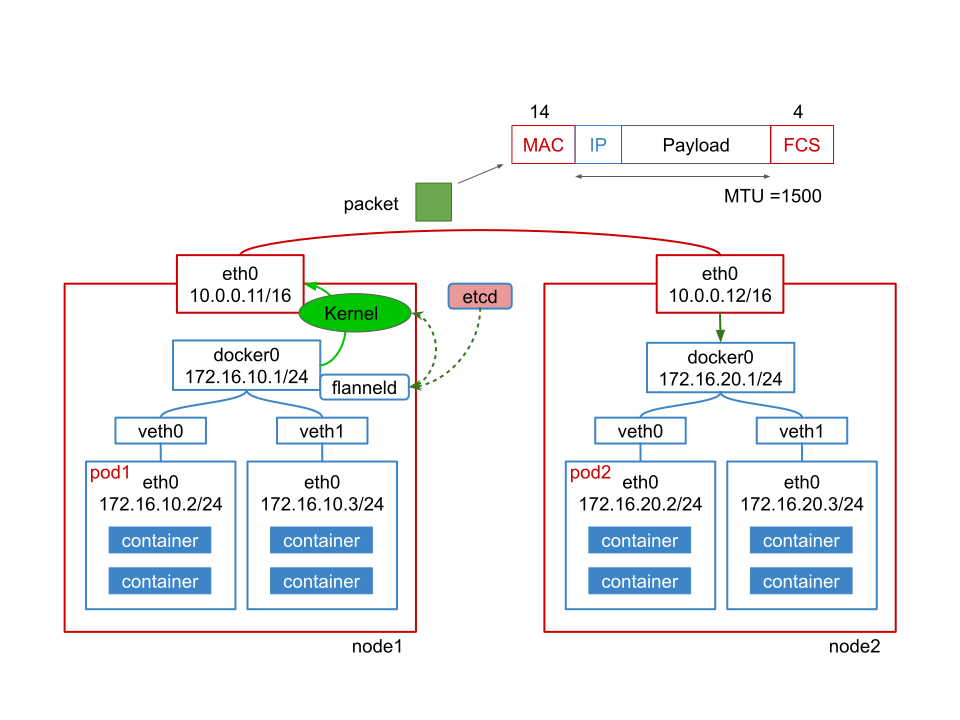
\includegraphics[width=0.95\columnwidth]{Figs/flannel-host-gw}

  \par\bigskip
  \centering
  \begin{minipage}{0.9\columnwidth}
    \caption[Flannel setup with host-gw mode]{
      Flannel setup with host-gw \added[id=4th]{mode}.
      \added[id=4th]{
      The {\em pod1} on the node1 sends out an IP packet to {\em pod2} on the node2.
      After receiving packets from the {\em pod1}, the node1 learns that {\em pod2} is on the node2, and forward the packets to the node2 without any encapsulation.
      The flanneld continuously updates routing entries for containers in the routing table on each node.
      }
    }
    \label{Figs/flannel-host-gw}
  \end{minipage}
\end{figure}

\FloatBarrier

\subsubsection{vxlan mode}

In the case of the vxlan mode, flanneld creates the Linux kernel's vxlan device, flannel.1. 
Flanneld will also configure\deleted[id=4th]{s} the routing table appropriately based on the information stored in the etcd.
When {\em pods} on different nodes need to communicate, the packet is routed to flannel.1.
The vxlan functionality of the Linux kernel identify the MAC address of flannel.1 device on the destination node with the help of flanneld, then form an Ethernet frame toward \replaced[id=4th]{that}{the} MAC address.
The vxlan then encapsulates the Ethernet frame in a UDP/IP packet with a vxlan header, after which the IP packet is eventually sent out.
An additional 50 bytes of header is used in the vxlan mode, thereby resulting in an MTU size of 1450 bytes.

\begin{figure}[h]
  \centering
  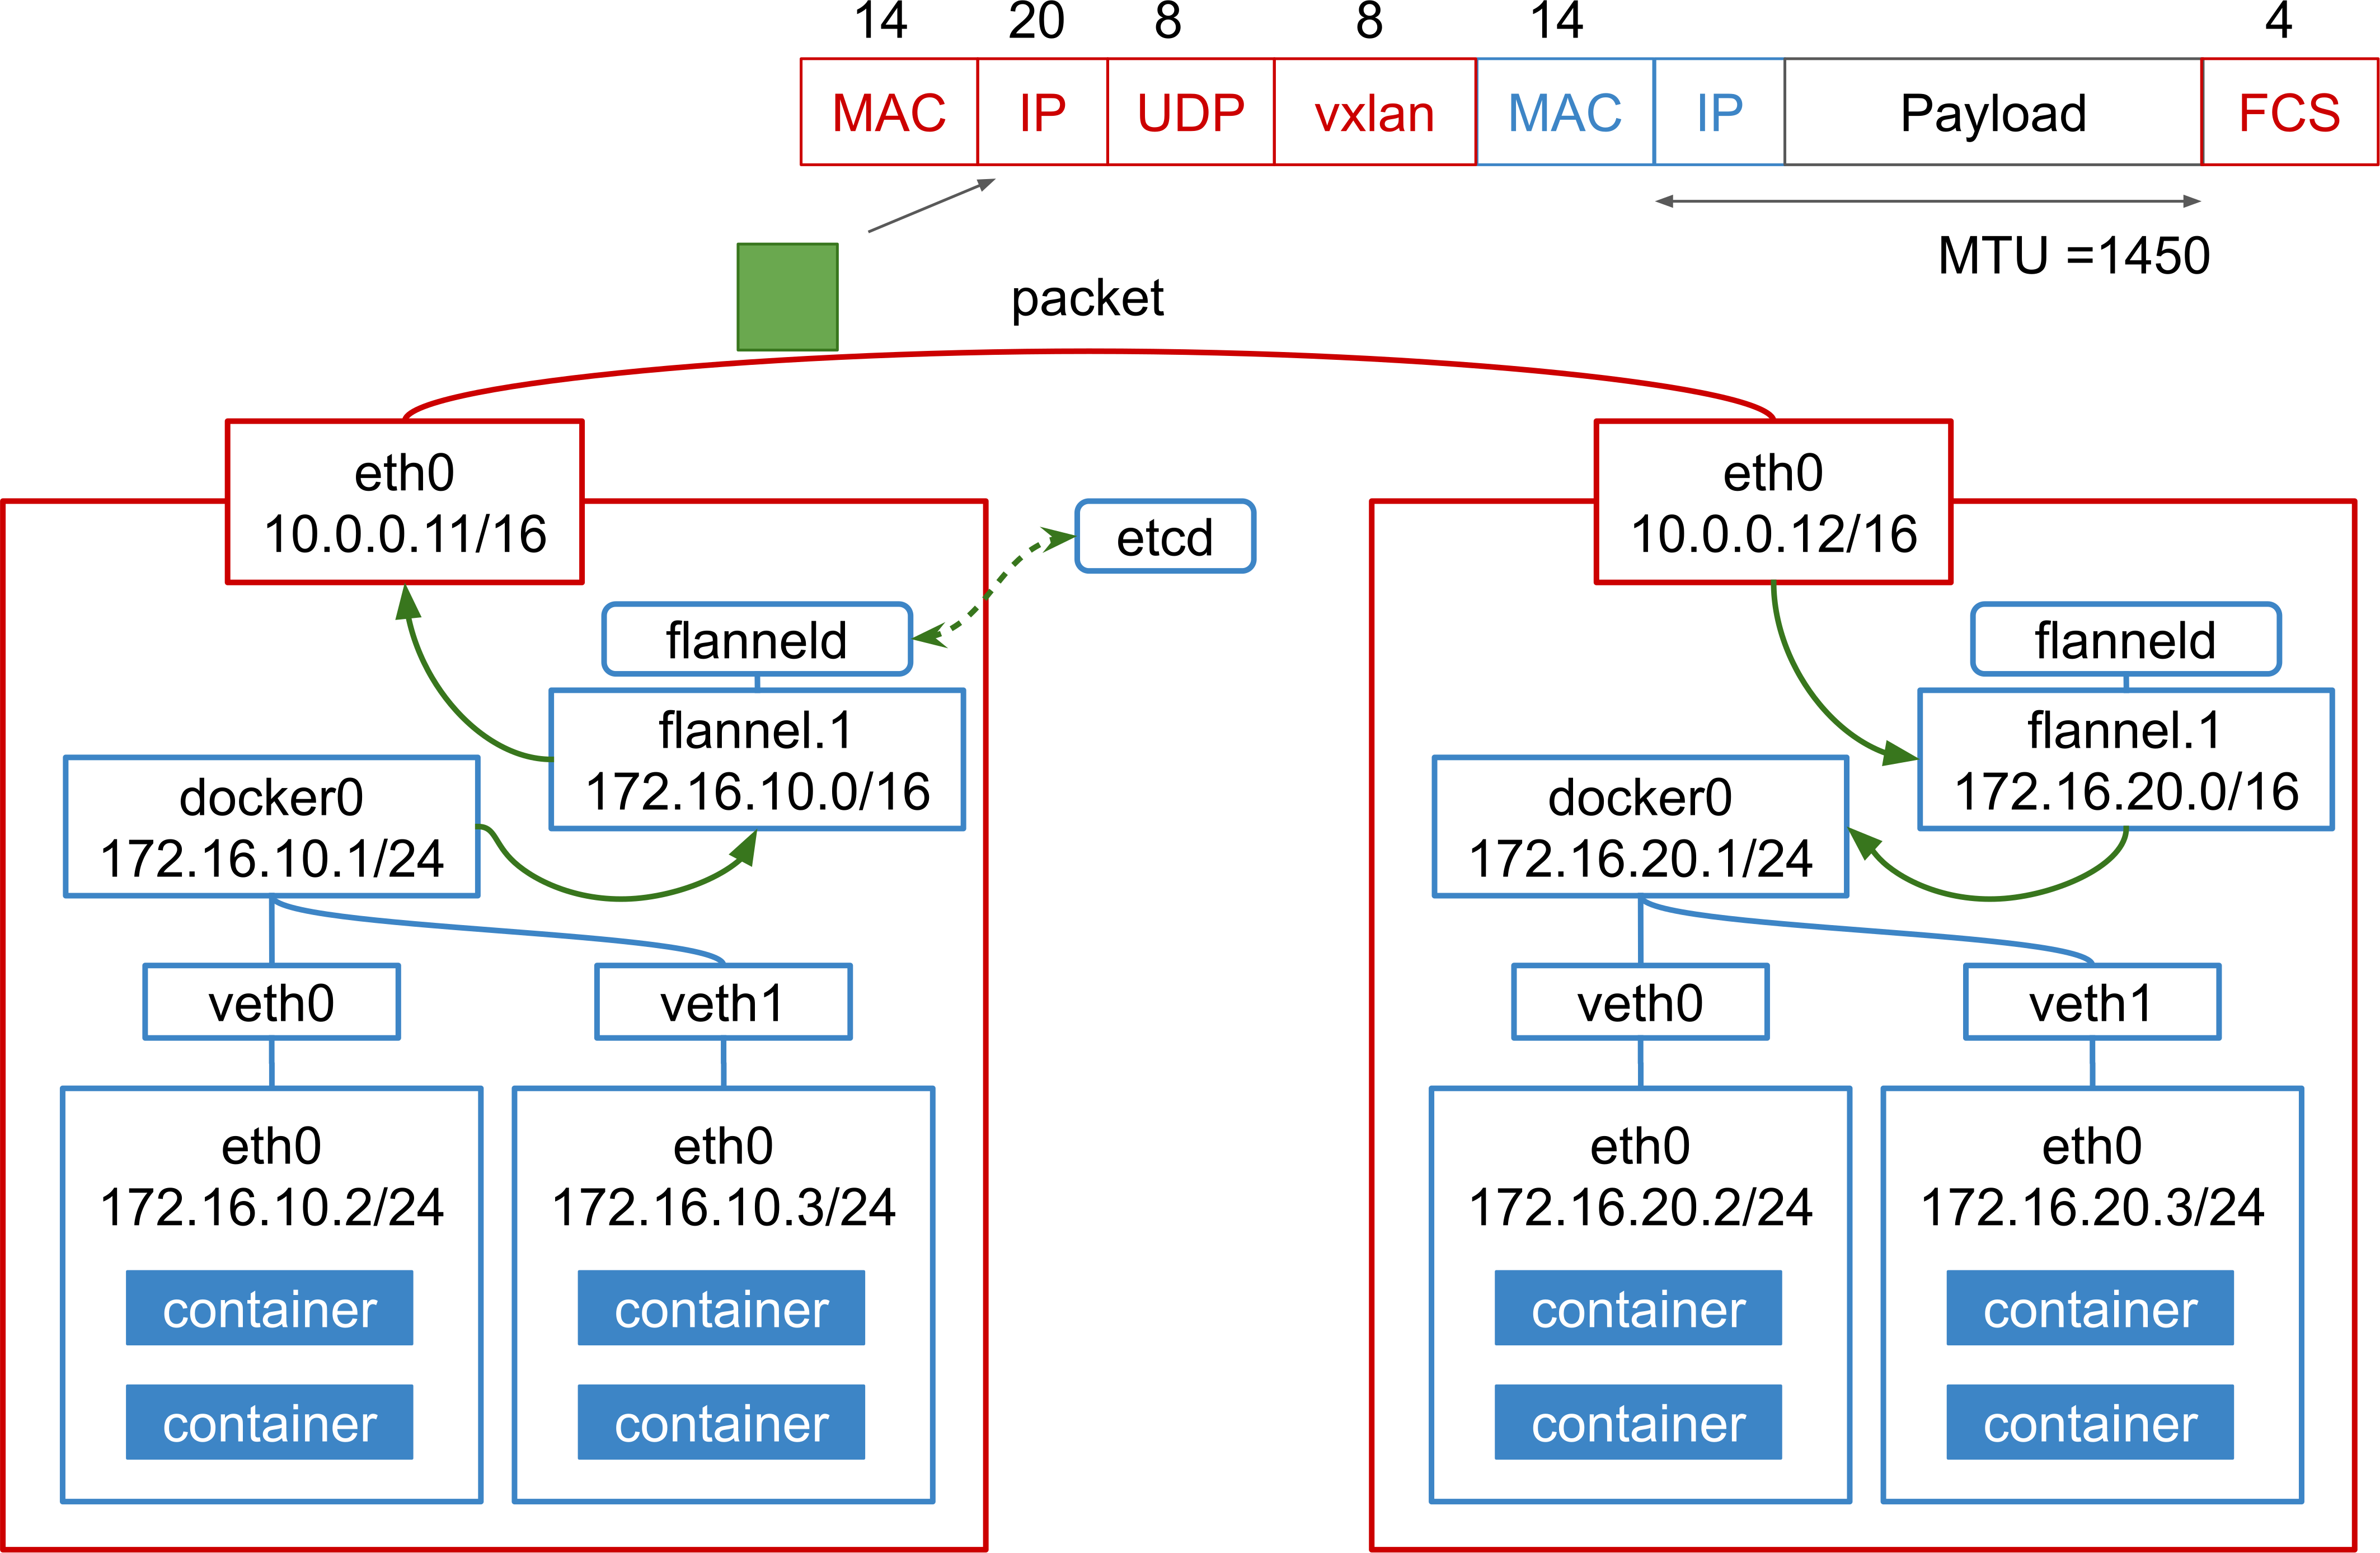
\includegraphics[width=0.95\columnwidth]{Figs/flannel-vxlan}

  \par\bigskip
  \centering
  \begin{minipage}{0.9\columnwidth}
    \caption[Flannel setup with vxlan]{
      Flannel setup with vxlan.
      \added[id=4th]{
      The flanneld on the nodes updates routing entries for containers.
      In addition to that, the flanneld also create Linux kernel's vxlan device, flannel.1 on every node.
      When packets are sent out through flannel.1 devices, the flannel.1 encapsulate the original packets with vxlan headers.
      }
    }
    \label{Figs/flannel-vxlan}
  \end{minipage}
\end{figure}

\FloatBarrier

\subsubsection{udp mode}

In the case of udp mode, flanneld creates the tun device, flannel0, and configures the routing table\added[id=4th]{ appropriately based on the information stored in the etcd}.
The flannel0 device is connected to the flanneld daemon itself.
An IP packet routed to flannel0 is encapsulated by flanneld, and eventually sent out 
to the appropriate node. 
The encapsulation is done for IP packets.
In the case of the udp mode, only 28 bytes of header are used for encapsulation, which results in an MTU size of 1472 bytes.

\begin{figure}[h]
  \centering
  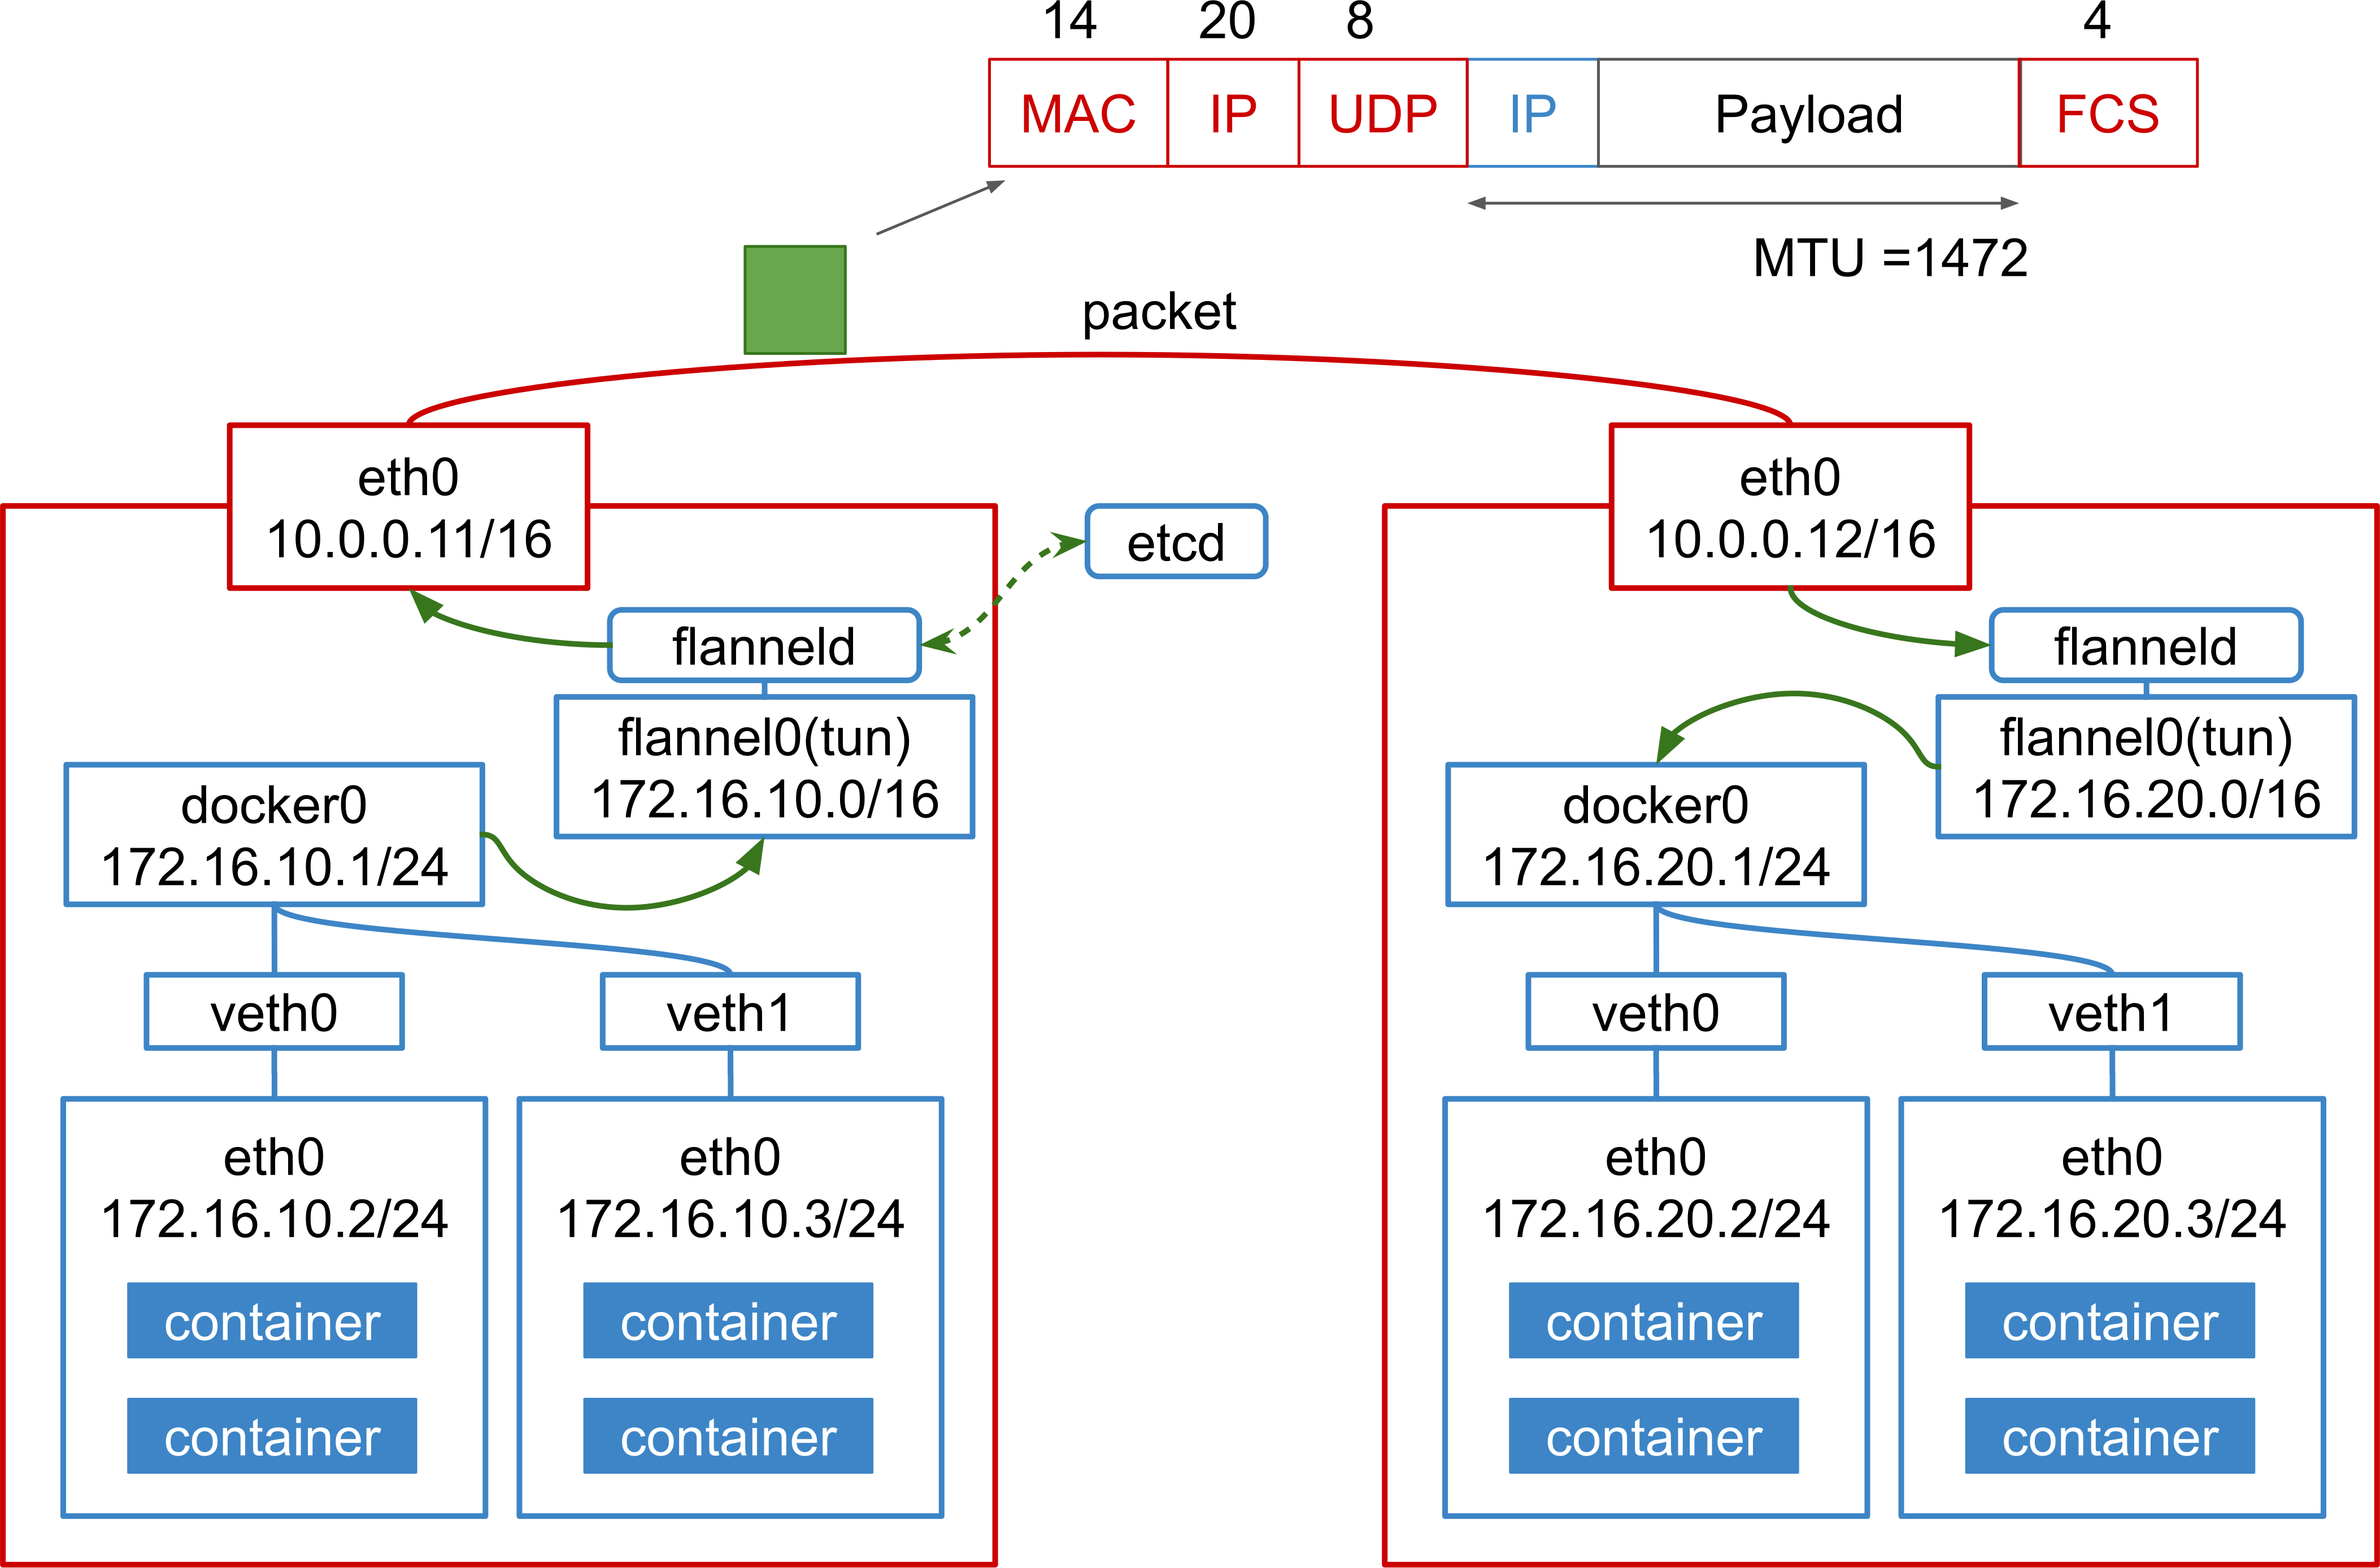
\includegraphics[width=0.95\columnwidth]{Figs/flannel-udp}

  \par\bigskip
  \centering
  \begin{minipage}{0.9\columnwidth}
    \caption[Flannel setup with udp]{
      Flannel setup with udp.
      \added[id=4th]{
      The flanneld creates the tun device, flannel0, and updates routing entries for containers.
      The flannel0 device is connected to the flanneld daemon itself.
      When packets are sent out through flannel0 devices, the flanneld daemon encapsulates the original packets with udp headers.
      }
    }
    \label{Figs/flannel-udp}
  \end{minipage}
\end{figure}

\FloatBarrier

\subsection{Caveats of the overlay network}

There are caveats in using overlay network.
The author explains two of them that are identified in the course of this study.


  The first is that overlay network without encapsulation has issues when used in cloud environments.
  There are chances when there is a gateway host without a knowledge of the overlay network between two containers.
  When such gateway host receive\replaced[id=4th]{s}{d} a packet destined to a container without encapsulation, it simply drops the packet because it does not know where to send it.

  The second is that there is an issue when two containers communicate with a host without knowledge of the ovelay network.
  Since the packets are translated using \replaced[id=4th]{SNAT}{Source Network Address Translation (SNAT) \cite{MartinA.Brown2017}}, the host can not identify if the two connections are coming from a single container or from two containers only by looking into IP and TCP headers.


\subsubsection{Overlay network and cloud}

Although the host-gw mode is expected to be most efficient since no packet encapsulation is used, it has a significant drawback that prohibit it to work correctly in cloud platforms. 
The host-gw mode simply sends out a packet without encapsulation.
If there is a cloud gateway between nodes, the gateway cannot identify the proper destination, therefore it drops the packet.

\begin{table}
  \centering
  \begin{tabular}{lccc}
    \toprule
    mode & On-premise & GCP & AWS \\
    \midrule
    host-gw & OK & NG & NG \\
    vxlan & OK & OK & OK \\
    udp & OK & OK & OK \\
    \bottomrule
  \end{tabular}

  \par\bigskip
  \centering
  \begin{minipage}{0.9\columnwidth}
    \caption[Flannel backend modes]{
      Flannel backend modes.
      The host-gw mode without encapsulation does not work in GCP nor in AWS.
    }
    \label{tab:Viable flannel backends}
  \end{minipage}
\end{table}

The author conducted an investigation to determine which of the flannel backend mode would be usable on AWS, GCP, and on-premise data centers.
The results are summarized in Table~\ref{tab:Viable flannel backends}. 
In the case of GCP, an IP address \added[id=4th]{with the prefix length of 32 (/32 in CIDR notation)}\deleted[id=4th]{ of {\tt /32}} is assigned to every VM host and every communication between VMs goes through GCP's gateway.
As for AWS, the VMs within the same subnet communicate directly, while the VMs in different subnets communicate via the AWS's gateway.
Since the gateways do not have knowledge of the flannel overlay network, they drop the packets; thereby, 
they prohibit the use of the flannel host-gw mode in those cloud providers.  

\subsubsection{Communication with router}

The overlay network also causes a problem when communicating with \replaced[id=4th]{the host that has no knowledge of}{a host that knows nothing about} the overlay network.
Fig.~\ref{fig:overlay} shows schematic diagram of network architecture of a container cluster system. 
There is a \replaced[id=4th]{node network (physical server network)}{physical network (node network)} with \added[id=4th]{the} IP address range of 10.0.0.0/16 and an overlay network with \added[id=4th]{the} IP address range of 172.16.0.0/16.
The node network is the network for nodes to communicate with each other.
The overlay network is the network setups for containers to communicate with each other.
An overlay network typically consists of appropriate routing tables on nodes, and optionally of tunneling setup using \replaced[id=4th]{IPIP}{ipip} \cite{kuznetsov1999tunnels} or vxlan \cite{zismer2016performance}.
The upstream router usually belongs to the node network.
When a container in the Fig.~\ref{fig:overlay} communicates with any of the nodes, it can use its IP address in 172.16.0.0/16 \deleted[id=4th]{IP }range as a source IP, since every node has proper routing table for the overlay network.
\replaced[id=4th]{However, when}{When} a container communicates with the upstream router that does not have routing information regarding the overlay network, the source IP address must be translated by \replaced[id=4th]{SNAT}{Source Network Address Translation (SNAT)} rules on the node \added[id=4th]{where} the container resides.

The SNAT caused a problem when the author tried to co-host multiple load balancer pods for different services on a single node and let them connect the upstream router directly.
This was due to the fact that the BGP agent used in our experiment only used the source IP address of the connection to distinguish the BGP peer.
The agent on the router behaved as though different BGP connections from different containers belonged to a single BGP session because the source IP addresses were identical due to the SNAT.

\begin{figure}[h]
  \centering
  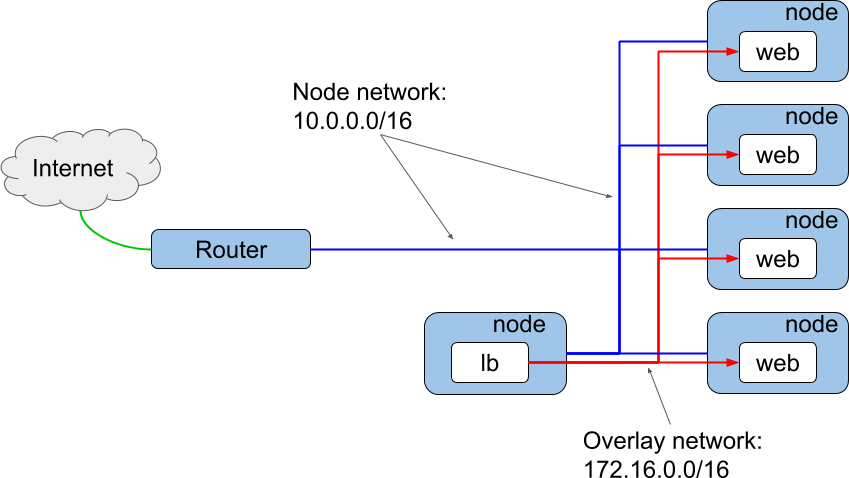
\includegraphics[width=0.95\columnwidth]{Figs/overlay.png}

  \par\bigskip
  \centering
  \begin{minipage}{0.9\columnwidth}
    \caption[A network architecture of container cluster system]{
      A network architecture of container cluster system.
      A load balancer (lb) pod (the white box with "lb") and web pods are running on nodes (the blue boxes).
      The traffic from the internet are forwarded to the lb pod by the upstream router using the node network,
      and the distributed to web pods using the overlay network.
    }
    \label{fig:overlay}
  \end{minipage}
  
\end{figure}

\FloatBarrier

\section{Multicore packet processing}

\added[id=4th]{
The Linux kernel comes with built-in features for multi-core packet processing.
However, the default setting of Linux distribution might not \replaced[id=4th]{be necessarily}{necessarily be} optimized for the best performance, which sometimes hinders the understanding of experimental results.
That was the case when the author first carried out the experiment, and therefore the author explains about it.
}

The performance of a computer system has been improved significantly thanks to the development of multi-core CPUs.
One of the top of the line server processors from Intel now includes up to 28 cores in a single CPU.
In order to enjoy the benefits of multi-core CPUs in communication performance,
it is necessary to distribute the handling of interrupts from the NIC and the \added[id=4th]{subsequent} IP protocol processing to the available physical cores.

Receive Side Scaling (RSS) \cite{TomHerbert} is a technology 
to distribute handling of the interrupt from NIC queues to multiple CPU cores.
\deleted[id=4th]{Subsequently, }Receive Packet Steering (RPS) \cite{TomHerbert} distributes the IP protocol processing 
to multiple CPU cores by issuing inter core software interrupts.

Since \replaced[id=4th]{performance levels of a load balancer}{load balancer performance levels} could be affected by these technologies,
the author conducted an experiment to determine how \replaced[id=4th]{performance levels of the load balancers are changed by}{ how load balancer performance level changes depending on} the RSS and RPS settings in Chapter~\ref{chapter:Performance Evaluation}.
The \replaced[id=4th]{lest of this section explains}{following shows} how RSS and RPS are enabled and disabled in the experiment. 
The NIC used in the experiment is Broadcom BCM5720, which has four rx-queues and one tx-queue.
Figure~\ref{fig:rx-queue} shows the interrupt request (IRQ) number assignments to those NIC queues at the time of experiments.

\begin{figure}[h]
\centering
\begin{minipage}{0.3\columnwidth}
\begin{verbatim}
81: eth0-tx-0
82: eth0-rx-1
83: eth0-rx-2
84: eth0-rx-3
85: eth0-rx-4
\end{verbatim}
\end{minipage}

\par\bigskip
\centering
\begin{minipage}{0.9\columnwidth}
  \caption[The IRQ numbers assigned for each RX/TX queue]{
    The IRQ numbers assigned for each RX/TX queue, which is obtained from \enquote{/proc/interrupts}.
    IRQ numbers from 81 to 85 are assigned to different tx and rx queues.
  }
  \label{fig:rx-queue}
\end{minipage}

\end{figure}

\subsubsection{RSS}

When packets arrive, they are distributed to these rx-queues depending on the flow each packet belongs to.
Each receive queue has a separate IRQ associated with it. The NIC triggers
this to notify a CPU when new packets arrive on the given queue.
Then, the notified CPU handles the interrupt, and performs the protocol processing. 
According to the \cite{TomHerbert}, the CPU cores allowed to be notified is controlled by setting a hexadecimal value corresponding to the bit maps indicating the allowed CPU cores in \enquote{/proc/irq/[IRQ number]/smp\_affinity}.
%
For example, in order to route the interrupt for eth0-rx-1 to CPU0, one should set \enquote{/proc/irq/82/smp\_affinity} to binary number {\tt 0001}, which is 1 in hexadecimal value.
Further\added[id=4th]{more}, in order to route the interrupt for eth0-rx-2 to CPU1, one should set \enquote{/proc/irq/83/smp\_affinity} to binary number {\tt 0010}, which is 2 in hexadecimal value.

In this dissertation,
\replaced[id=4th]{the setting that distributes interrupts from four rx-queues separately to CPU0, CPU1, CPU2, and CPU3 is referred to as}{the author refers to the setting to distribute interrupts from four rx-queues to CPU0, CPU1, CPU2, and CPU3 as} \enquote{RSS = on}.
It is configured as the setting in Figure~\ref{fig:rss=on}.
%
On the other hand, \enquote{RSS = off} means that \replaced[id=4th]{all the interrupts}{an interrupt} from any rx-queue \replaced[id=4th]{are}{is} routed to CPU0. 
It is configured as the setting in Figure~\ref{fig:rss=off}.

\begin{figure}[h]

  \begin{subfigure}[t]{\columnwidth}
    \centering
    \begin{minipage}{0.6\columnwidth}
\begin{verbatim}
echo 1 > /proc/irq/82/smp_affinity
echo 2 > /proc/irq/83/smp_affinity
echo 4 > /proc/irq/84/smp_affinity
echo 8 > /proc/irq/85/smp_affinity
\end{verbatim}
    \end{minipage}
    \caption{\underline{\textbf{RSS=on}}}
    \label{fig:rss=on}
  \end{subfigure}

  \par\bigskip

  \begin{subfigure}[t]{\columnwidth}
    \centering
    \begin{minipage}{0.6\columnwidth}
\begin{verbatim}
echo 1 > /proc/irq/82/smp_affinity
echo 1 > /proc/irq/83/smp_affinity
echo 1 > /proc/irq/84/smp_affinity
echo 1 > /proc/irq/85/smp_affinity
\end{verbatim}
    \end{minipage}
    \caption{\underline{\textbf{RSS=off}}}
    \label{fig:rss=off}
  \end{subfigure}

  \par\bigskip
  \centering
  \begin{minipage}{0.9\columnwidth}
    \caption[RSS settings]{
      RSS settings used in this study.
      \added[id=4th]{
      (a) This setting distributes interrupts from the IRQ\# 82--85 to CPU0--CPU3, respectively.
      (b) This setting directs all the interrupts from IRQ\# 82--85 to CPU0.
      }
    }
    \label{fig:rss_settings}
  \end{minipage}

  \par\bigskip
\end{figure}

\subsubsection{RPS}

\added[id=4th]{
After the interrupts from the NIC are handled, IP protocol processings are carried out.
}
The RPS distributes IP protocol processing by placing the packet
on the desired CPU's backlog queue and wakes up the CPU using inter-processor interrupts.
The author \replaced[id=4th]{has}{have} used the settings in Figure~\ref{fig:rps=on} to enable the RPS.

\begin{figure}[h]

  \begin{subfigure}[t]{\columnwidth}
    \centering
    \begin{minipage}{0.9\columnwidth}
\begin{verbatim}
echo fefe > /sys/class/net/eth0/queues/rx-0/RPS_cpus
echo fefe > /sys/class/net/eth0/queues/rx-1/RPS_cpus
echo fefe > /sys/class/net/eth0/queues/rx-2/RPS_cpus
echo fefe > /sys/class/net/eth0/queues/rx-3/RPS_cpus
\end{verbatim}
    \end{minipage}
    \caption{\underline{\textbf{RPS=on}}}
    \label{fig:rps=on}
  \end{subfigure}

  \par\bigskip

  \begin{subfigure}[t]{\columnwidth}
    \centering
    \begin{minipage}{0.9\columnwidth}
\begin{verbatim}
echo 0 > /sys/class/net/eth0/queues/rx-0/RPS_cpus
echo 0 > /sys/class/net/eth0/queues/rx-1/RPS_cpus
echo 0 > /sys/class/net/eth0/queues/rx-2/RPS_cpus
echo 0 > /sys/class/net/eth0/queues/rx-3/RPS_cpus
\end{verbatim}
    \end{minipage}
    \caption{\underline{\textbf{RPS=off}}}
    \label{fig:rps=off}
  \end{subfigure}

  \par\bigskip
  \centering
  \begin{minipage}{0.9\columnwidth}
    \caption[RPS settings]{
      RPS settings used in this study.
      \added[id=4th]{
      (a) IP protocol proccessings are distributed to CPU1--CPU7 and CPU9--CPU15.
      (b) Distribution of IP protocol proccessings is prohibitted.
      Original CPUs that recieved interrupts will process the IP protocols.
      }
    }
    \label{fig:rps_settings}
  \end{minipage}

  \par\bigskip
\end{figure}

Since the hexadecimal value \enquote{fefe} represented as \enquote{1111 1110 1111 1110} in binary, 
this setting will \replaced[id=4th]{distribute}{allow distributing} protocol processing to all of the CPUs, except for CPU0 and CPU8.
The CPU0 and CPU8 are logically different but share the same physical core\footnote{\added[id=4th]{The hardware used in the experiment had Hyper-Threading functionality \cite{marr2002hyper}, therefore each of the physical cores are shared by two logical cores.}}.
In this dissertation, the author refers to this setting as \enquote{RPS = on}.
%
On the other hand, \enquote{RPS = off} means that no CPU is allowed for RPS. 
\replaced[id=4th]{In this case}{Here}, the IP protocol processing is performed on the CPUs the initial hardware interrupt is received.
It is configured as the settings in Figure~\ref{fig:rps=off}.

The RPS is especially effective when the NIC does not have multiple receive queues or when the number of queues is 
much smaller than the number of CPU cores. 
That was the case in the experiment\deleted[id=4th]{, where the NIC had only four rx-queues, while there was a CPU with eight physical cores}.
\added[id=4th]{
Since there were only four rx-queues, RSS could utilize only four physical cores out of eight.
}
Figure~\ref{Figs/rss-rps-none} shows a schematic diagram of the setting\added[id=4th]{s} used in this study.
While merely enabling RSS results in four core packet processing, enabling RPS results in eight \added[id=4th]{physical} core packet processing.

\begin{figure}[h]
  \centering
  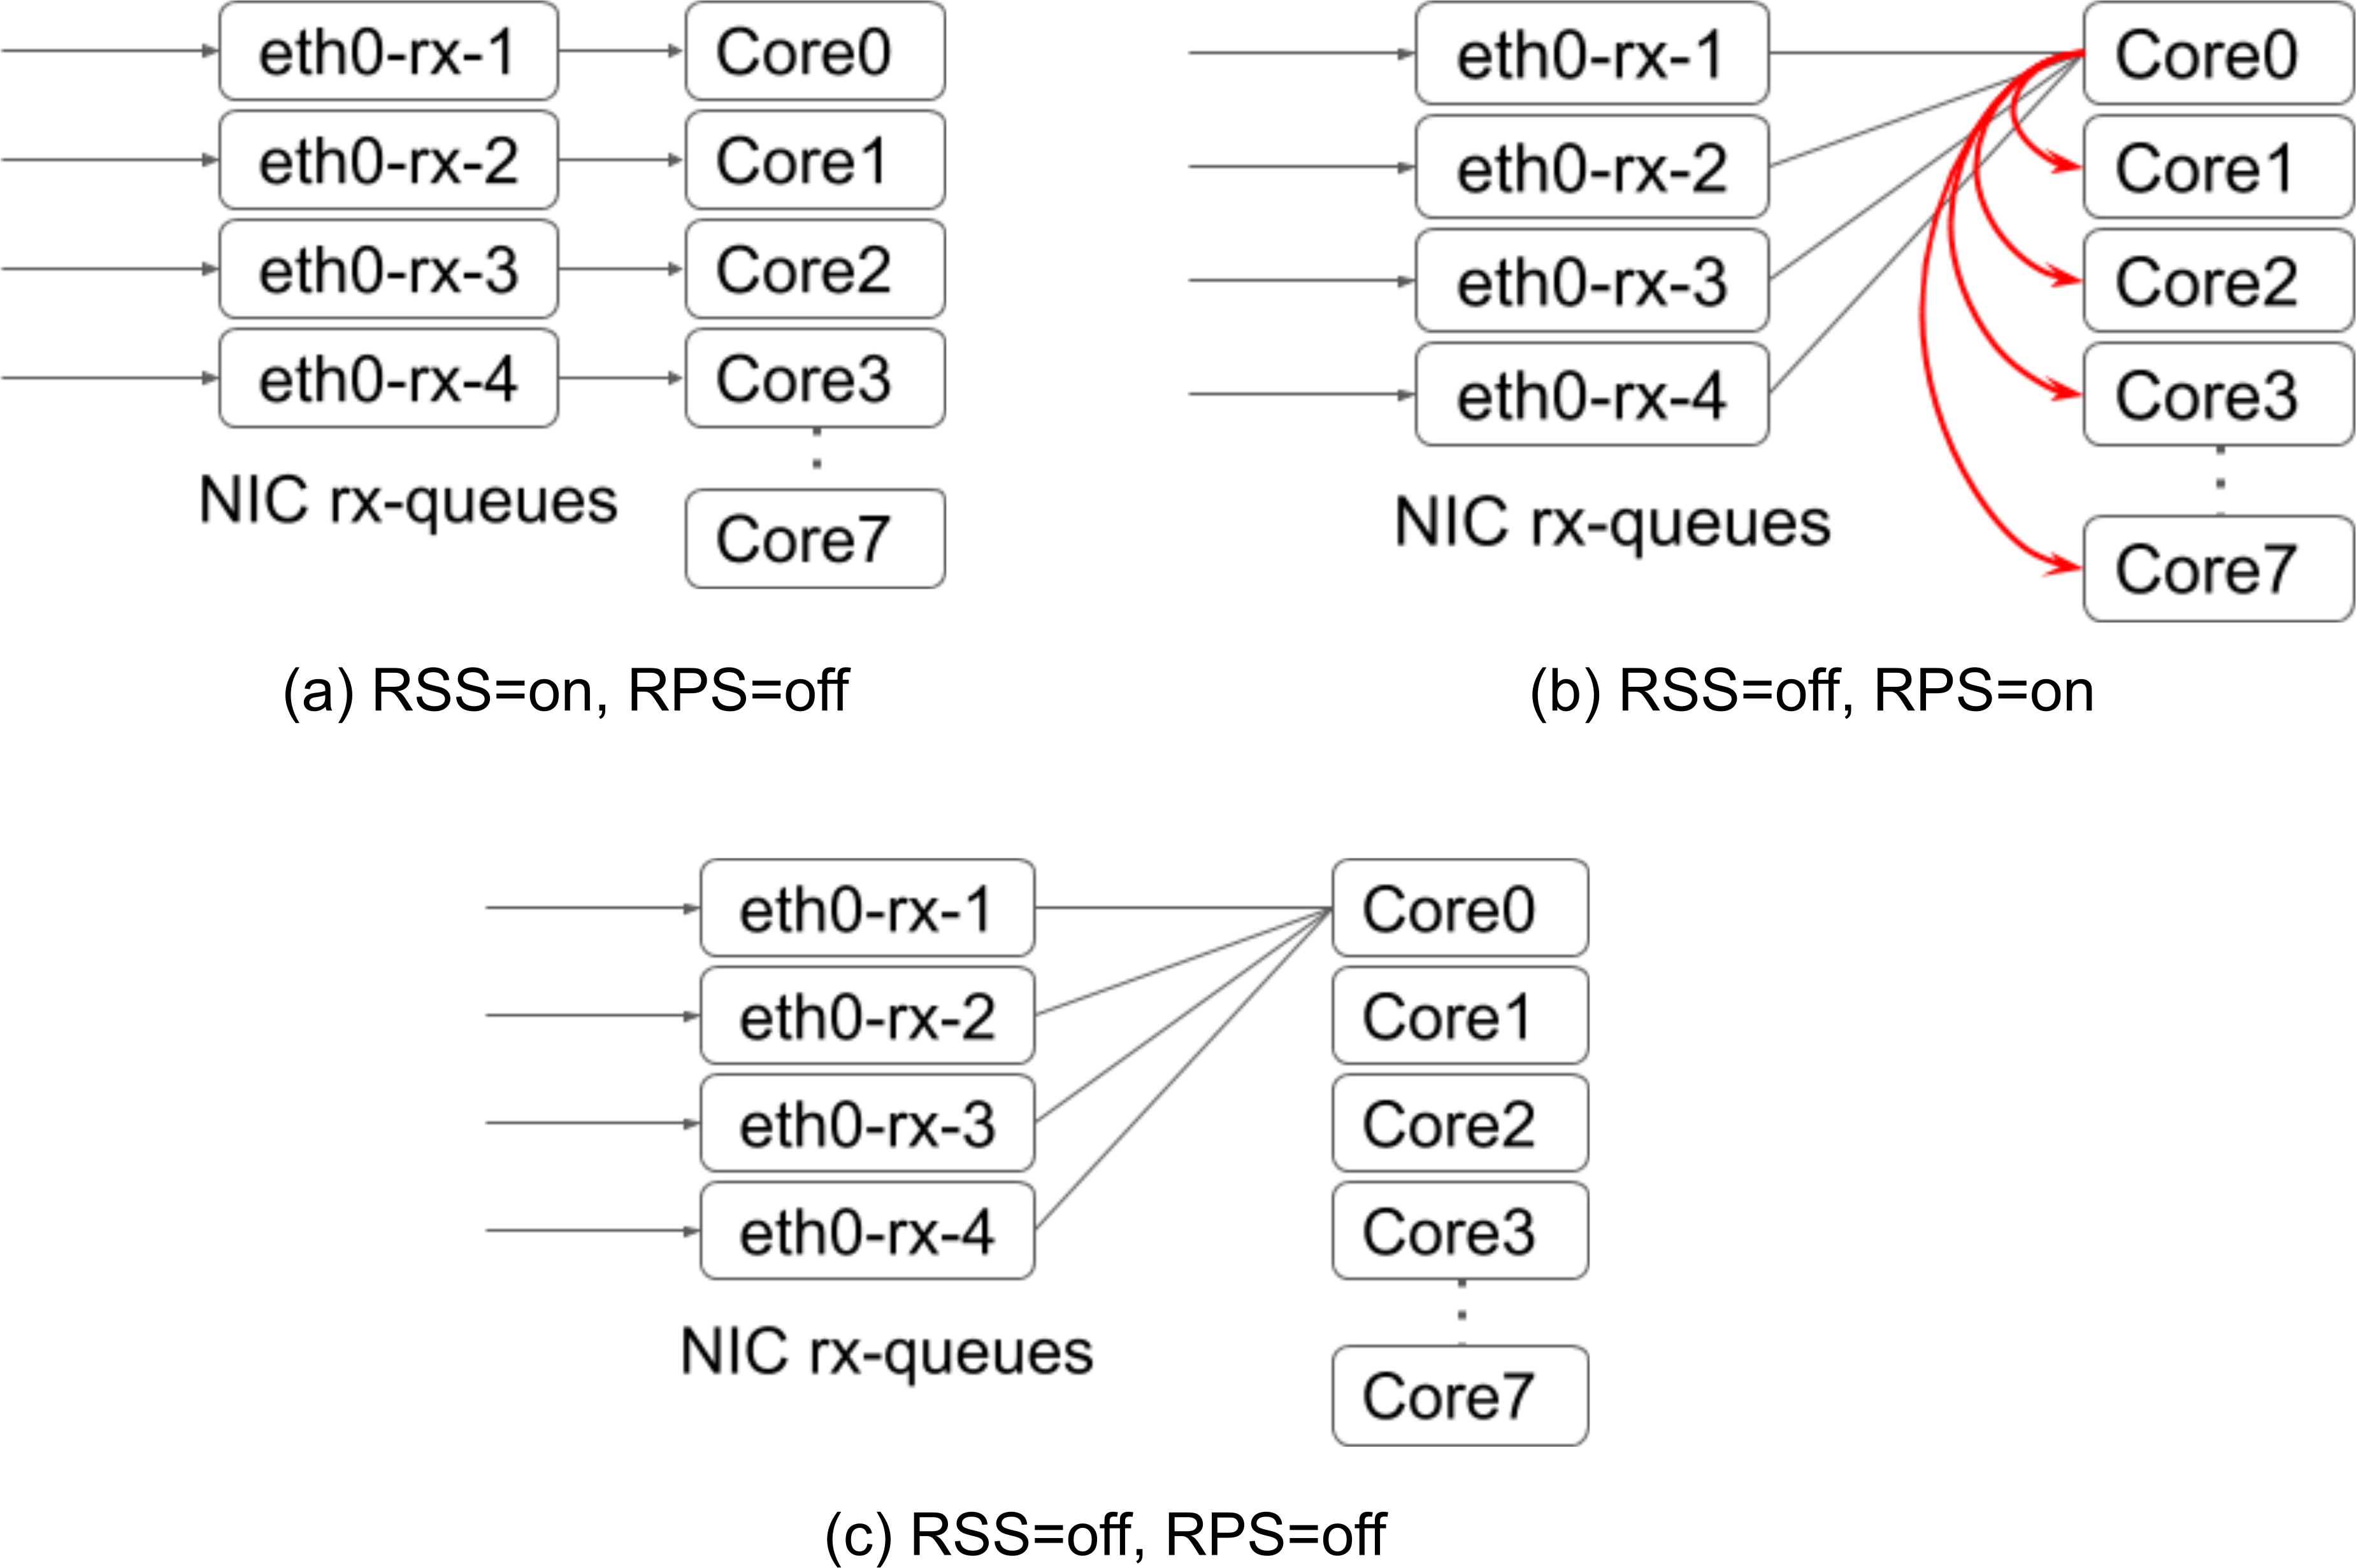
\includegraphics[width=0.95\columnwidth]{Figs/rss-rps-none}

  \par\bigskip
  \centering
  \begin{minipage}{0.9\columnwidth}
    \caption[RSS/RPS settings]{
      RSS/RPS settings used in this study.
      (a) In the case of \enquote{RSS=on,RPS=off}, \added[id=4th]{only} four cores are used for packet processing.
      (b) In the case of \enquote{RSS=off,RPS=on}, eight cores are used for packet processing.
      (c) In the case of \enquote{RSS=off,RPS=off}, \replaced[id=4th]{only one}{single} core is used for packet processing.
    }
    \label{Figs/rss-rps-none}
  \end{minipage}
\end{figure}

\FloatBarrier

\section{IPVS load balancer}

The IPVS is a Layer-4 load balancer capability, which is included in the Linux kernel 2.6.0 released in 2003 or later, 
to distribute incoming Transmission Control Protocol (TCP) traffic \added[id=4th]{and User Datagram Protoco (UDP) traffic} to 
{\em real server}s\footnote{The term, {\em real server} refers to worker servers that will respond to incoming traffic, 
in the original literature \cite{Zhang2000}. \replaced[id=4th]{The author}{We} will also use this term in the similar way.} \cite{Zhang2000}. 
For example, IPVS distributes incoming Hypertext Transfer Protocol (HTTP) traffic destined for a single destination IP address, to multiple HTTP servers\deleted[id=4th]{ (e.g. Apache HTTP or nginx)} running on multiple nodes in order to improve the performance of web services.
\added[id=4th]{The destination IP address is often called Virtual IP (VIP) because the VIP and the multiple HTTP servers form a virtual service.}
The IPVS has three \replaced[id=4th]{operation modes}{mode of operation}, Network Address Translation (NAT), Tunneling and (Direct Return) DR.
In this study the author used NAT mode and Tunneling mode.
Here the author explains \replaced[id=4th]{these two modes}{them} briefly\footnote{\added[id=4th]{Readers interested in the DR mode, are referred to the original literature \cite{Zhang2000}.}}.

\subsection{NAT mode}

\begin{figure}[h]
  \centering
  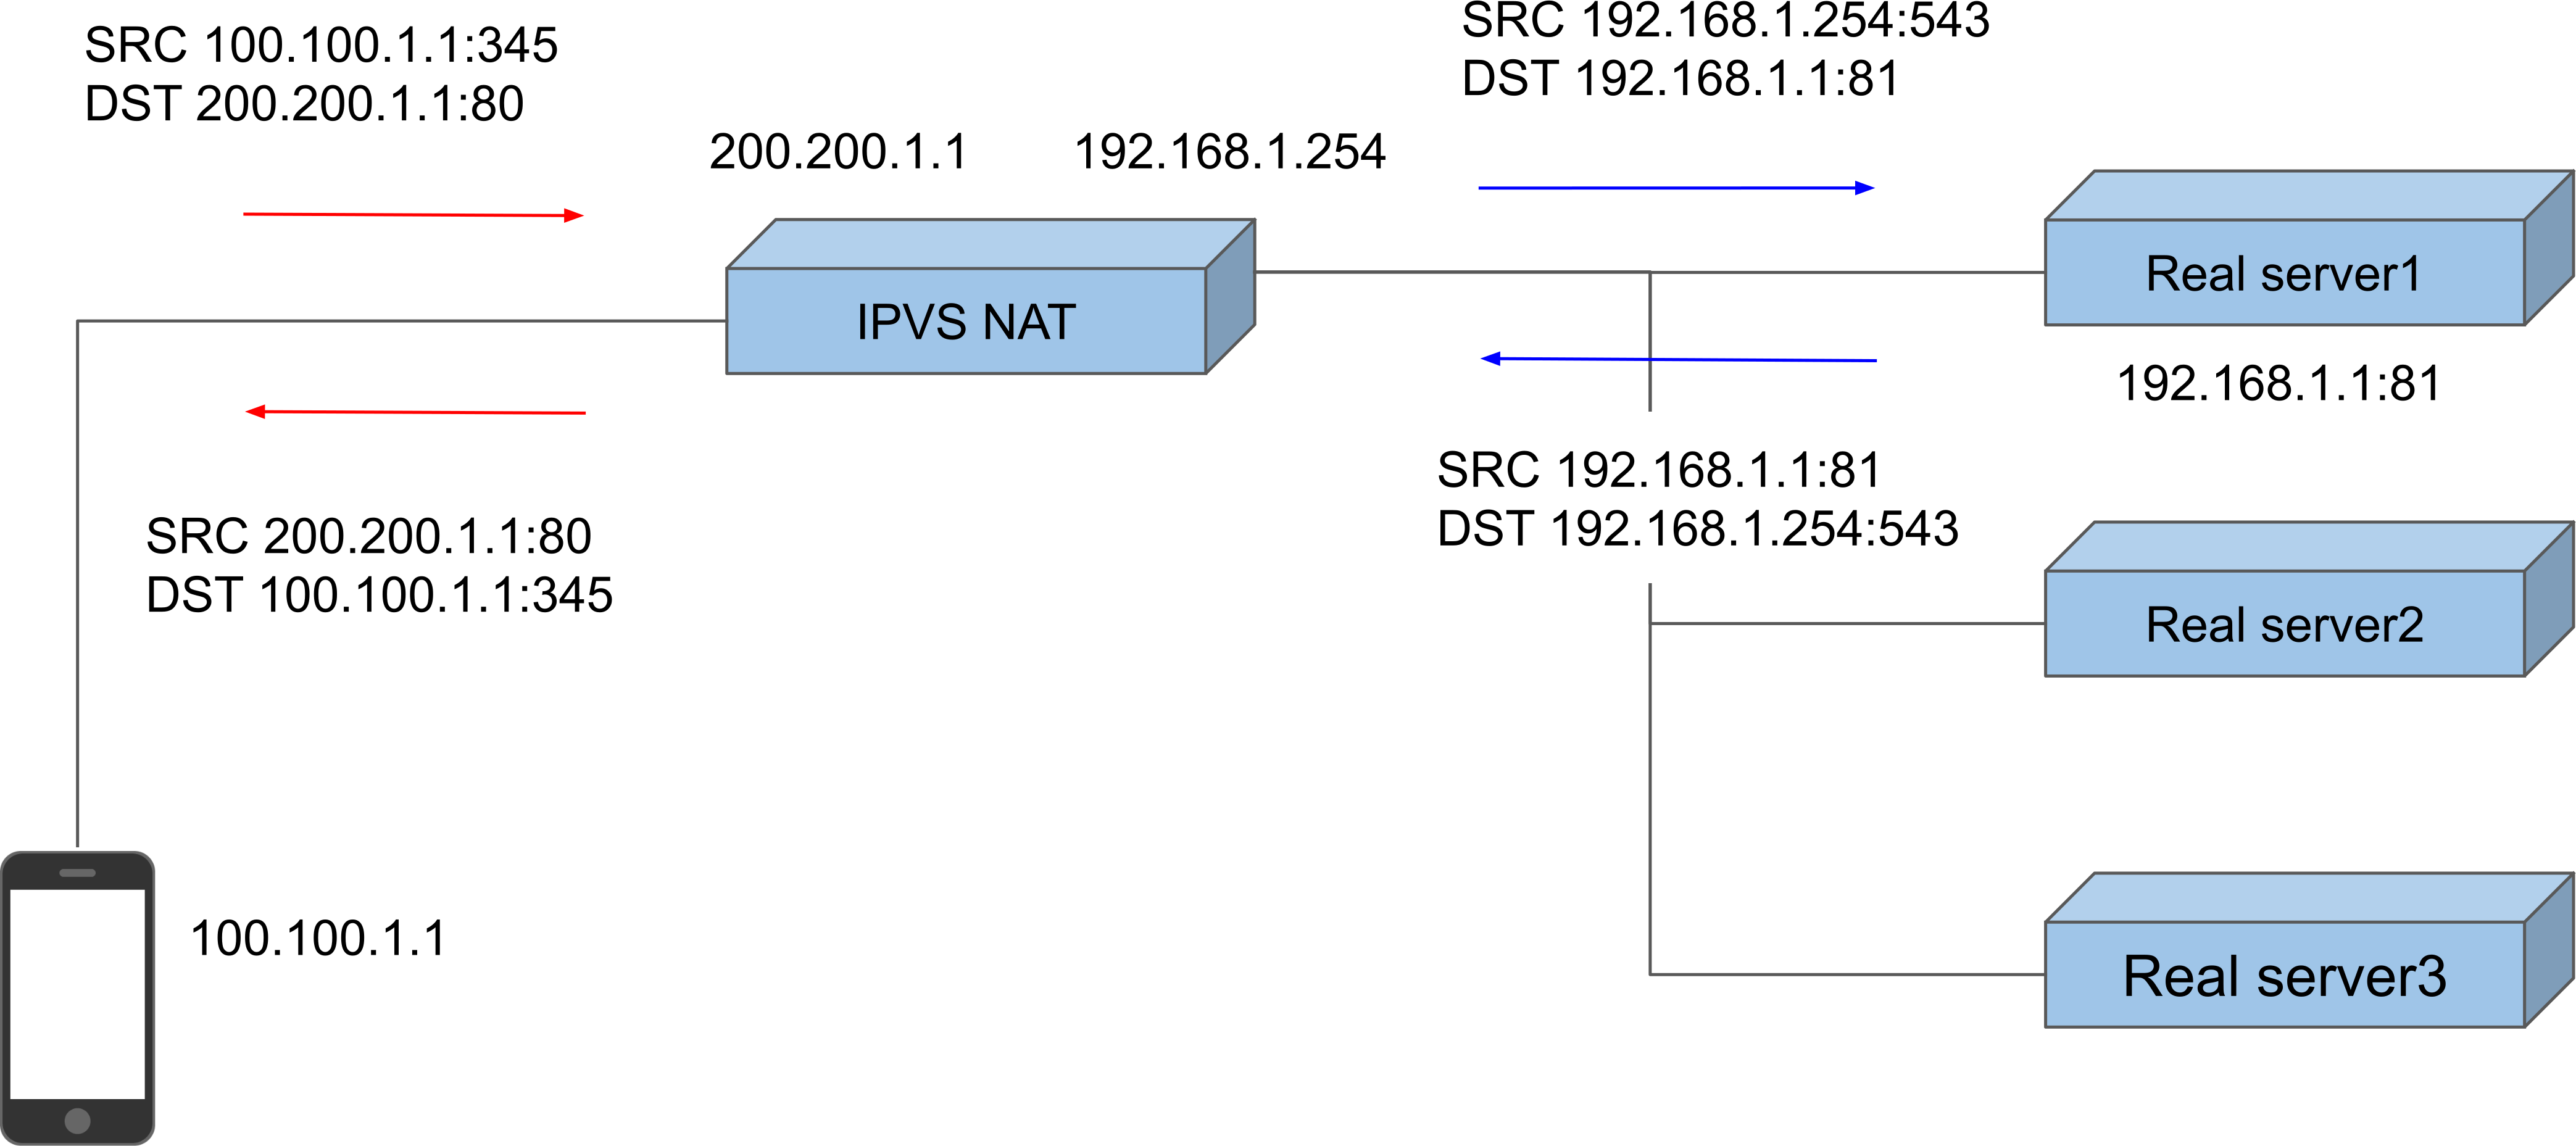
\includegraphics[width=0.95\columnwidth]{Figs/ipvs-nat-schem}

  \par\bigskip
  \centering
  \begin{minipage}{0.9\columnwidth}
    \caption[IPVS NAT mode]{
    Schematic diagram of IPVS NAT mode.
    \added[id=4th]{
    The IP packets arriving at the IPVS NAT enabled host are forwarded to real servers.
    The IP headers are translated by IPVS NAT function in the Linux kernel.
    }
    }
    \label{fig:ipvs-nat-schem}
  \end{minipage}
\end{figure}

Figure~\ref{fig:ipvs-nat-schem} shows a schematic diagram of NAT mode of IPVS.
The NAT mode works as follows: When a user accesses a virtual service provided by the server cluster, a request packet destined for \replaced[id=4th]{a VIP}{virtual IP address (the IP address to accept requests for virtual service)} arrives at the load balancer.
The load balancer examines the packet's destination address and port number, if they \replaced[id=4th]{match}{are matched for} a virtual service \replaced[id=4th]{in the load balancing table}{according to the virtual server rule table}, \replaced[id=4th]{one of the}{a} real server\replaced[id=4th]{s are}{ is} selected \replaced[id=4th]{depending on the}{from the cluster by a} scheduling algorithm, and \added[id=4th]{the information regarding} the connection is added into the \added[id=4th]{connection} hash table\deleted[id=4th]{ which records connections}. 
Then, the destination \added[id=4th]{IP} address and the port \added[id=4th]{number} of the \added[id=4th]{original} packet are \replaced[id=4th]{translated}{rewritten} to those of the \replaced[id=4th]{real}{selected} server, and the packet is forwarded to the \added[id=4th]{real} server. 
When an incoming packet belongs to an established connection, the connection can be found in the hash table and the packet \replaced[id=4th]{is}{will be} rewritten and forwarded to the right server. 
When response packets \replaced[id=4th]{arrive}{come back}, the load balancer rewrites the source address and port \added[id=4th]{number} of the packets to those of the virtual service\added[id=4th]{, and send them back to the clients}.
When a connection terminates or timeouts, \replaced[id=4th]{the corresponding entry is}{ the connection record will be} removed \replaced[id=4th]{from the connection}{in the} hash table.
%
\replaced[id=4th]{In this dissertation, the}{ The} author refers to this NAT mode simply as IPVS hereafter\deleted[id=4th]{ in this dissertation}.

\FloatBarrier

\subsection{Tunneling mode}

\begin{figure}[h]
  \centering
  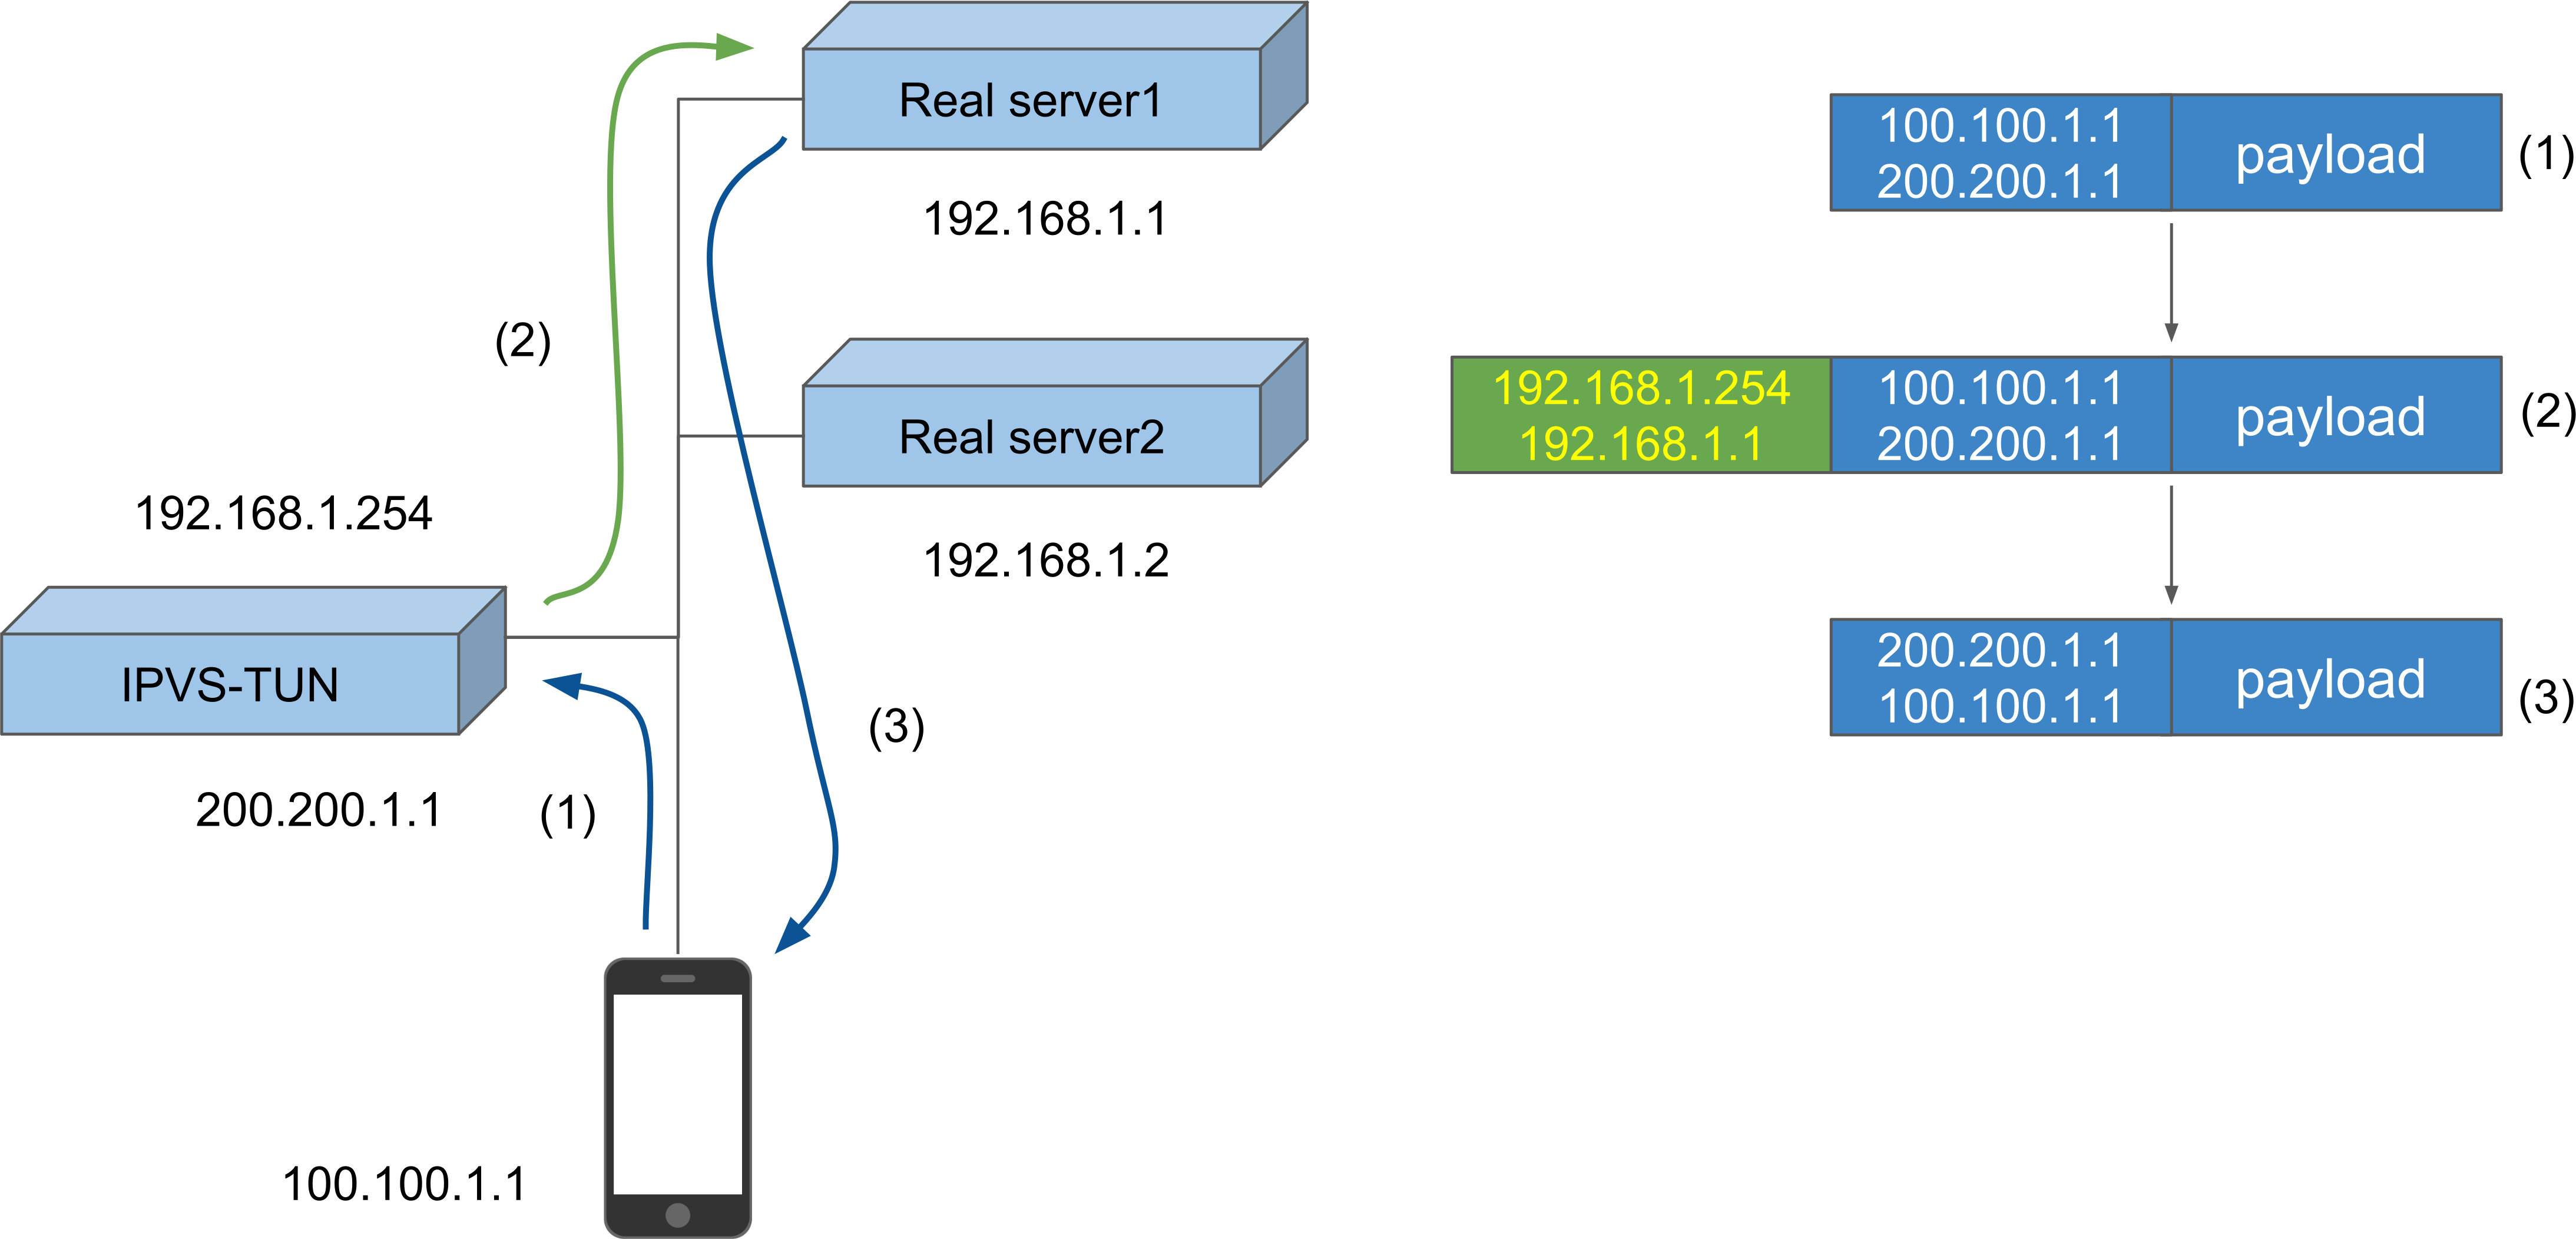
\includegraphics[width=0.95\columnwidth]{Figs/ipvs-tun-schem}

  \par\bigskip
  \centering
  \begin{minipage}{0.9\columnwidth}
    \caption[IPVS tunneling  mode]{
    Schematic diagram of IPVS tunneling mode.
    \added[id=4th]{
    (1) The packet arriving IPVS-TUN enabled host is encapsulated and (2) sent out to one of the real servers.
    (3) The real server returns the response packets to the client directly. 
    }
    }
    \label{fig:ipvs-tun-schem}
  \end{minipage}
\end{figure}

Figure~\ref{fig:ipvs-tun-schem} shows a schematic diagram of \added[id=4th]{the} tunneling mode of IPVS.
IP\added[id=4th]{IP} tunneling (IP encapsulation) is a technique to encapsulate IP datagram within IP datagram\replaced[id=4th]{.}{,}
\replaced[id=4th]{This technique}{which} allows datagrams destined for one IP address to be wrapped and redirected to another IP address \cite{kuznetsov1999tunnels}\deleted[id=4th]{.
This technique}\added[id=4th]{, and} can be used to build a virtual server\added[id=4th]{.}
\replaced[id=4th]{The}{that the} load balancer \replaced[id=4th]{encapsulates}{tunnels} the request packets \added[id=4th]{and sends them out} to the \replaced[id=4th]{real}{different} servers,
and the \added[id=4th]{real} servers \added[id=4th]{decapsulate and} process the requests\replaced[id=4th]{, and then}{ and} return the results to the clients directly\replaced[id=4th]{.}{,}
\replaced[id=4th]{As a result,}{thus} the service can still appear as a virtual service on a single IP address.

In the tunneling mode of the IPVS, the load balancer encapsulates the packet within an IP datagram and forwards it to a dynamically \replaced[id=4th]{selected}{elected} server. 
When the \added[id=4th]{real} server receives the encapsulated packet, it decapsulates the packet and finds the inside packet is destined for VIP that is on its tunnel device\deleted[id=4th]{, so it processes the request, and returns the result to the client directly}.
\added[id=4th]{Therefore, the real server can return response packets originating from VIP directly to the clients.
It should be noted that in the NAT mode, the real servers never know VIP.
}
%
The author refers to the tunneling mode of the IPVS as IPVS-TUN hereafter\deleted[id=4th]{,} in this dissertation.

\FloatBarrier

\section{XDP technology}

In Chapter~\ref{chapter:Further Improvement} \replaced[id=4th]{the}{this} author implements a software load balancer using eXpress Data Path (XDP) \cite{hoiland2018express} technology.
Here the XDP is briefly explaned.

XDP is a framework to enable injection of a byte-compiled eBPF programs into the NIC driver, so that the program can manipulate a received packet \added[id=4th]{at the} earliest point in the Linux networking stack.
Therefore much better performance than conventional Linux kernel's network stack is expected.
\added[id=4th]{One can create their eBPF program by writing codes in C and then compiling them with Clang using the -march=bpf parameter.}
\deleted[id=4th]{One can write his own eBPF program in C by compiling with Clang using the -march=bpf parameter.}
The eBPF program injected into the Kernel is just-in-time compiled and used for packet manipulation.
XDP merely intercept and process packets only if the packets match the conditions.
The packets that \replaced[id=4th]{do}{did} not match the condition are passed through conventional Linux kernel network stack.
Therefore there is no need for preparing dedicated NIC for fast and efficient network processing.
\added[id=4th]{This is one of the advantages of the XDP technology, compared with the technology using Data Plane Development Kit (DPDK) \cite{dpdkorg}.}
Use cases for XDP include DDoS protection, packet forwarding, and load balancing, flow sampling, monitoring, etc.

\begin{figure}[h]
  \centering
  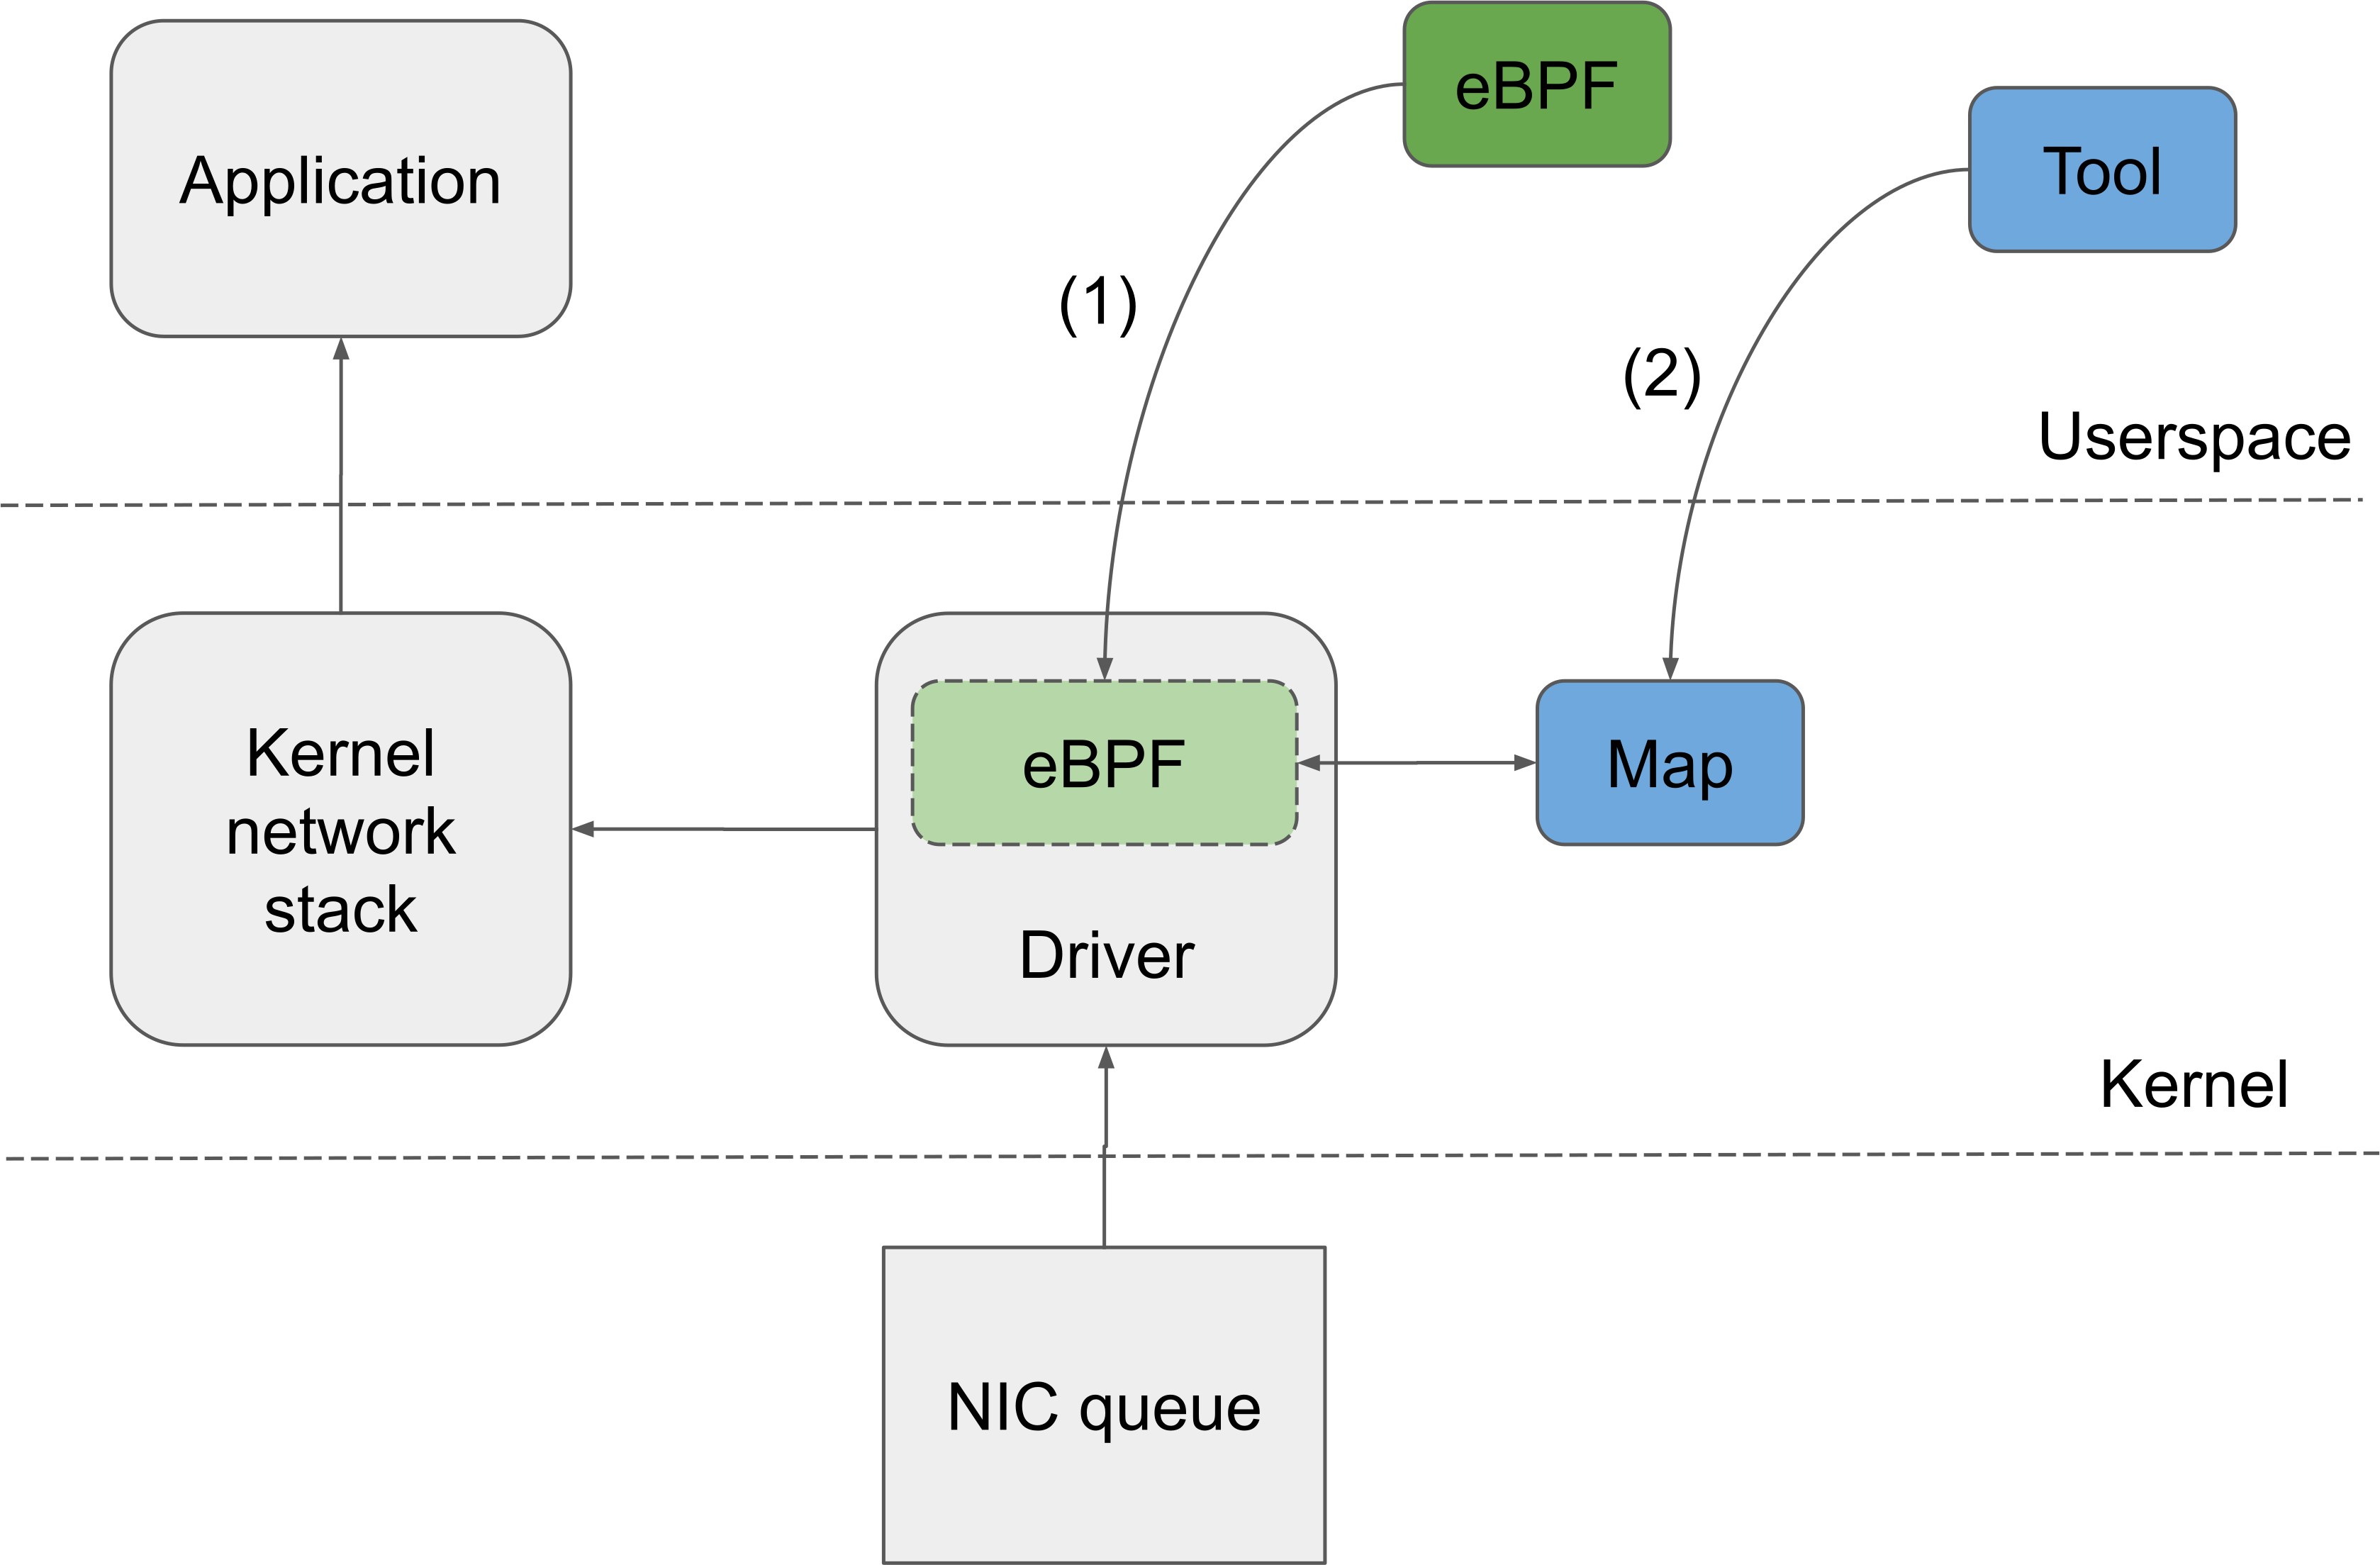
\includegraphics[width=0.95\columnwidth]{Figs/xdp-schem}

  \par\bigskip
  \centering
  \begin{minipage}{0.9\columnwidth}
    \caption[XDP architecture]{
      XDP architecture.
      In XDP, user can inject self-made byte-compiled eBPF code in the NIC driver and let it process the incoming packets much earlier than the kernel's network stack.
      The eBPF programs can make a map inside the kernel, and read/store temporal data from that map.
      The map is mount at \enquote{/sys/fs/bpf/}.
      User can manipulate the behaviour of the eBPF through this map.
    }
    \label{fig:xdp-schem}
  \end{minipage}
\end{figure}

\FloatBarrier

\section{Summary}

This chapter provided explanations of the following technologies; 1) Overlay network 2) Multicore packet processing 3) IPVS load balancer 4) XDP technology.
These are the underlying technologies used in this study, and knowledge of these is necessary to understand the contents of this thesis.

Overlay networks are used to deploy Kubernetes clusters, and its operation mode greatly affects the throughput of the load balancers.
\added[id=4th]{Therefore, they have been explained here.}
The Linux kernel comes with built-in features for multi-core packet processing.
However, the setting might not be optimized for the best performance, and lack of knowledge might hinder the understanding of the experimental results.
\added[id=4th]{Therefore, this technology has also been explained.}
The Linux kernel's IPVS is also necessary to be understood because this is one of the core \replaced[id=4th]{technologies}{technology} used in this study\added[id=4th]{, and thus included here}.
The author plans to replace IPVS based load balancer with the one based on XDP technology in order to improve the performance to meet 100 Gbps level in future work.
The explanation of XDP technology is \added[id=4th]{also} necessary to understand why it is supposed to be faster than IPVS.

